\documentclass{ctexart}
\usepackage{amsmath, amssymb}
\usepackage{geometry}
\usepackage{hyperref}
\usepackage{verbatim}
\usepackage{listings}
\usepackage{xcolor}
\usepackage{tikz}
\usepackage{graphicx}
\usetikzlibrary{shapes, arrows, positioning, automata, shadows, fit}

\lstdefinestyle{cpp}{%
    language=C++,
    basicstyle=\footnotesize\ttfamily,
    keywordstyle=\color{blue},
    stringstyle=\color{red},
    commentstyle=\color{green},
    numbers=left,
    numberstyle=\tiny\color{gray},
    stepnumber=1,
    numbersep=5pt,
    backgroundcolor=\color{white},
    showspaces=false,
    showstringspaces=false,
    showtabs=false,
    frame=single,
    rulecolor=\color{black},
    tabsize=2,
    captionpos=b,
    breaklines=true,
    breakatwhitespace=false,
    title=\lstname,
    morekeywords={Matrix, Point2D, Vector, Polygon_2, CDT, Criteria, Mesher}
}
\lstset{style=cpp}

\geometry{a4paper, margin=1in}

\title{\texttt{CrossSection2dFEM} 中声学模式的有限元分析及其在软件架构中的作用}
\author{基于 VocalTractLab3D 代码分析 (Blandin et al., 2022 [1])}
\date{\today}

\begin{document}

\maketitle

\section{引言}
在 VocalTractLab3D 框架中,\texttt{CrossSection2dFEM} 类负责表示声道的任意二维横截面,并计算其声学特性。根据 Blandin et al.~(2022 [1]) 的描述,该软件采用结合多模态方法和有限元 (FEM) 的策略。其中,\textbf{二维有限元方法 (2D FEM) 的核心作用是计算声道各个横截面的横向声学模式 (transverse modes, $\phi_n$)},这些模式随后被用于构建多模态传播模型,以模拟声波在考虑曲率和截面积变化的声道中的传播。

本文档的目的在于详细解析 \texttt{CrossSection2d.cpp} 中,特别是 \texttt{CrossSection2dFEM::computeModes} 函数内实现的 2D FEM 计算过程,阐明其如何根据论文 [1] 的理论计算出横向模式以及后续多模态分析所需的耦合矩阵,并说明其在整体软件架构中的位置。

\section{软件架构概述 (基于 Blandin et al., 2022 [1])}
VocalTractLab3D 的核心模拟架构基于 Blandin 等人 [1] 提出的高效 3D 声学模拟方法,其主要特点是结合了二维有限元(2D FEM)和多模态传播技术。其基本流程和架构可以概括为以下几个关键阶段:

\begin{enumerate}
    \item \textbf{几何处理与分段 (Geometry Processing \& Segmentation)}
        \begin{itemize}
            \item \textit{输入:} 接受 3D 声道几何形状,可以是由 VocalTractLab 内置的发音模型生成,也可以是从外部文件(如 MRI 数据转换而来)导入。
            \item \textit{处理:} 将连续的 3D 声道沿中心线 (centerline) 切割成一系列短的\textbf{段 (segments)}。关键假设是:在每一段内部,其\textbf{横截面形状保持不变},但允许其面积和位置(曲率)沿段的轴向变化。这种分段是应用多模态方法的基础 (论文 Sec. II.A, Fig. 1)。
            \item \textit{实现:} 这部分功能主要由 \texttt{VocalTract.cpp} 类及其依赖项处理,负责计算中心线、法线、截面轮廓等。
        \end{itemize}

    \item \textbf{横向模式计算 (Transverse Mode Computation via 2D FEM)}
        \begin{itemize}
            \item \textit{目的:} 对每个分段的代表性二维横截面,精确计算其横向声学模式 $\phi_n$ (特征函数) 和对应的特征值 $\gamma_n^2$(决定截止频率)。这些模式构成了后续声场分解的基础。
            \item \textit{方法:} 采用 \textbf{2D 有限元方法 (FEM)} 求解该横截面上的亥姆霍兹特征值问题(论文 Eq. 31),使用 Neumann 边界条件。
            \item \textit{实现:} \textbf{本文档后续章节将详细解析此步骤的实现},位于 \texttt{CrossSection2dFEM::computeModes} 函数中,利用 CGAL 进行网格划分,利用 Eigen 求解 FEM 产生的广义特征值问题。
        \end{itemize}

    \item \textbf{计算多模态耦合矩阵 (Multimodal Coupling Matrices)}
        \begin{itemize}
            \item \textit{目的:} 基于 FEM 计算得到的模式 $\phi_n$,预先计算一系列积分矩阵 (C, D, E, KR2, DR)。这些矩阵量化了模式之间由于声道几何(如曲率 $\kappa$、横截面坐标 z、边界类型 s)和物理效应(如壁面损耗 $\zeta_n$)引起的耦合。
            \item \textit{方法:} 通过将 FEM 计算的中间矩阵(如质量矩阵、刚度矩阵、边界积分矩阵等)投影到模式基上获得(对应本文件 \eqref{eq:C_matrix}-\eqref{eq:KR2_matrix})。
            \item \textit{实现:} 这部分计算同样在 \texttt{CrossSection2dFEM::computeModes} 中,紧随特征值求解之后进行。\textbf{本文档后续章节也将详细解析这些矩阵的计算。}
        \end{itemize}

    \item \textbf{计算段间连接/散射矩阵 (Junction/Scattering Matrices)}
        \begin{itemize}
            \item \textit{目的:} 描述声波在相邻两个具有不同截面形状或面积的段的界面处的散射和模式转换。
            \item \textit{方法:} 通过计算模式匹配积分得到模式转换矩阵 F (论文 Eq. 44),并推导出阻抗/导纳在界面处的转换关系 (论文 Eq. 45-46)。论文提到,为了处理非包含截面的情况,可能引入零长度的交集截面段。
            \item \textit{实现:} 相关逻辑可能分布在 \texttt{Acoustic3dSimulation.cpp} (如 \texttt{computeJunctionMatrices} 或类似函数) 和 \texttt{CrossSection2dFEM.cpp} (存储和提供 F 矩阵)。
        \end{itemize}

    \item \textbf{轴向多模态传播 (Axial Multimodal Propagation)}
        \begin{itemize}
            \item \textit{目的:} 模拟声波(表示为各模式幅值向量 $\mathbf{p}$ 和辅助场 $\mathbf{q}$)沿分段声道轴向 $x$ 的传播。
            \item \textit{方法:} 求解一个耦合的一阶常微分方程组(见本文件 \eqref{eq:ode_coupled}),其系数矩阵 $\mathbf{M}(x)$ 由之前计算的多模态矩阵 (C, D, E, KR2) 以及物理参数和几何参数($k, l(x), l'(x), \kappa$ 等)构成。数值求解采用 Magnus-Möbius 格式(论文 Eq. 47-52),可以处理变化的截面积和曲率。
            \item \textit{实现:} 这部分核心的传播计算逻辑位于 \texttt{Acoustic3dSimulation.cpp} (如 \texttt{propagateMagnus} 或 \texttt{propagateImpedAdmit} 函数) 和 \texttt{CrossSection2dFEM.cpp} (实现具体的传播步骤)。
        \end{itemize}

    \item \textbf{边界条件与激励 (Boundary Conditions \& Excitation)}
        \begin{itemize}
            \item 在声门端(起始端)施加声源激励(如单位体积速度源)。
            \item 在口端(末端)施加辐射条件(如通过数值积分计算的辐射阻抗矩阵 ZoutNs, 论文 Eq. 53)或简化的边界条件(硬壁、零压力等)。
            \item 壁面损耗通过边界导纳系数 $\zeta$ 或 $\zeta_n$ 体现在传播方程中(见本文件 \eqref{eq:K2_matrix} 和 \eqref{eq:bc_q})。
            \item \textit{实现:} 边界条件的处理和声源的施加逻辑主要在 \texttt{Acoustic3dSimulation.cpp} 中。
        \end{itemize}

    \item \textbf{结果合成与输出 (Result Synthesis \& Output)}
        \begin{itemize}
            \item 整个流程通常用于计算频率响应(传递函数 H(f), 论文 Eq. 56)或特定频率下的声场分布(论文 Eq. 54)。
            \item 通过组合不同频率的计算结果,可以合成声音信号。
            \item \textit{实现:} \texttt{Acoustic3dSimulation.cpp} 负责协调计算并提供结果接口,GUI 部分(如 \texttt{Acoustic3dPage.cpp})或其他调用者获取这些结果进行显示或处理。
        \end{itemize}
\end{enumerate}

\textbf{总结:} 该架构的核心优势在于,通过 FEM 精确捕捉复杂横截面的模式特性,然后利用高效的多模态方法处理轴向传播,同时能够计入曲率和面积变化的影响,从而在计算效率和几何精度之间取得了良好的平衡,超越了传统的 TLM 和纯 FEM 方法。

\section{理论基础:考虑曲率和面积变化的波动方程 (对应论文 Sec. II.B)}
为了在多模态框架下处理弯曲且截面积变化的声道段,需要进行坐标变换并将波动方程转换到新的坐标系下。

\subsection{几何变换 (对应论文 Sec. II.B.1)}
引入一个从物理笛卡尔坐标 $(X,Y,Z)$ 到一个局部坐标系 $(x,y,z)$ 的变换。在这个局部坐标系中,声道段是直的且截面积恒定(参考形状)。$x$ 是沿着声道中心线的弧长坐标,$y, z$ 是局部横截面坐标。中心线在 $(X,Y,Z)$ 空间中的位置向量为 $\mathbf{s}(x)$,局部横截面基向量为 $\mathbf{n}_y, \mathbf{n}_z$(构成 Frenet-Serret 标架的一部分)。引入一个缩放因子 $l(x)$ 来描述截面尺寸沿 $x$ 的变化。一个物理点 $\mathbf{m}$ 的位置可以表示为:
\begin{equation} \label{eq:coord_transform}
\mathbf{m} = X \mathbf{i} + Y \mathbf{j} + Z \mathbf{k} = \mathbf{s}(x) + yl(x) \mathbf{n}_{y} + zl(x) \mathbf{n}_{z}.
\end{equation}
其中 $\mathbf{t} = d\mathbf{s}/dx$ 是中心线的切向量,$\kappa(x)$ 是中心线的曲率。假设弯曲发生在 $(X,Z)$ 平面内,即 $\mathbf{n}_y = \mathbf{j}$ 且 $\mathbf{n}_z$ 在 $(X,Z)$ 平面内与 $\mathbf{t}$ 正交,则有 $d\mathbf{n}_y/dx = 0$ 和 $d\mathbf{n}_z/dx = -\kappa(x) \mathbf{t}$。

通过微分 Eq. \eqref{eq:coord_transform} 并整理,可以得到两个坐标系之间的 Jacobian 矩阵 $\mathbf{J} = \frac{\partial (x, y, z)}{\partial (X, Y, Z)}$。其行列式为 $\det \mathbf{J} = 1/(fl^2)$,其中 $f(x, z) = 1 - z \kappa(x) l(x)$ 是一个与曲率相关的因子,$l' = dl/dx$。

\subsection{变换后的波动方程 (对应论文 Sec. II.B.2)}
原始的亥姆霍兹方程为 $(\Delta_X + k^2)p = 0$,其中 $\Delta_X$ 是笛卡尔坐标下的拉普拉斯算子,$k = \omega/c$ 是波数。利用坐标变换关系,可以将拉普拉斯算子变换到 $(x,y,z)$ 坐标系下:
\[
\Delta_X p = \det(\mathbf{J}) \text{div}(\mathbf{H} \boldsymbol{\nabla} p)
\]
其中 $\boldsymbol{\nabla} = (\partial_x, \partial_y, \partial_z)^T$ 是新坐标系下的梯度算子,$\text{div}$ 是对应的散度算子,而 $\mathbf{H}$ 是度量张量相关的矩阵:
\begin{equation} \label{eq:H_matrix}
\mathbf{H} = \frac{\mathbf{J}^T \mathbf{J}}{\det \mathbf{J}} = \frac{1}{f}
\begin{pmatrix}
l^2 & -yl'l & -zl'l \\
-yl'l & f^2 + (yl')^2 & yzl'^2 \\
-zl'l & yzl'^2 & f^2 + (zl')^2
\end{pmatrix}.
\end{equation}
变换后的波动方程为:
\begin{equation} \label{eq:wave_transformed}
\text{div}(\mathbf{H} \boldsymbol{\nabla} p) + \frac{k^2}{\det \mathbf{J}}p = \text{div}(\mathbf{H} \boldsymbol{\nabla} p) + k^2 f l^2 p = 0.
\end{equation}
同样,壁面边界条件 $\boldsymbol{\nabla}_X p \cdot \mathbf{n}_X + jk\zeta p = 0$(其中 $\mathbf{n}_X$ 是物理外法线,$\zeta = Z_0/Z_w$ 是归一化壁面导纳)变换为:
\begin{equation} \label{eq:bc_transformed}
\mathbf{H} \boldsymbol{\nabla} p \cdot \mathbf{n} + jk\zeta p = 0, \quad \text{for } y,z \in \Gamma_W,
\end{equation}
其中 $\mathbf{n}$ 是 $(x,y,z)$ 坐标系下的外法线,$\Gamma_W$ 是管壁。

\subsection{一阶演化方程形式}
为了得到关于轴向坐标 $x$ 的演化方程,引入辅助场 $q$,定义为声压梯度在 $\mathbf{H}$ 度量下的轴向分量:
\begin{equation} \label{eq:q_definition}
q \equiv (\mathbf{H} \boldsymbol{\nabla} p) \cdot \mathbf{t}_{local} = \frac{l}{f} (l \partial_x p - yl' \partial_y p - zl' \partial_z p),
\end{equation}
其中 $\mathbf{t}_{local} = (1, 0, 0)^T$ 是 $(x,y,z)$ 坐标系下的轴向单位向量。将 Eq. \eqref{eq:wave_transformed} 展开并代入 $q$ 的定义,可以得到关于 $(p, q)^T$ 的一阶偏微分方程组:
\begin{align} \label{eq:pde_first_order}
\partial_x
\begin{pmatrix} p \\
q \end{pmatrix}
&=
\begin{pmatrix}
\frac{l'}{l} \mathbf{v} \cdot \boldsymbol{\nabla}_\perp & \frac{f}{l^2} \\
-\text{div}_\perp(f \boldsymbol{\nabla}_\perp) - f(kl)^2 & \frac{l'}{l} \text{div}_\perp(\mathbf{v} \cdot)
\end{pmatrix}
\begin{pmatrix} p \\
q \end{pmatrix} ,
\end{align}
其中 $\mathbf{v} = (y, z)^T$ 是横向坐标向量,$\boldsymbol{\nabla}_\perp = (\partial_y, \partial_z)^T$ 是横向梯度算子,$\text{div}_\perp$ 是横向散度算子。相应的,变换后的边界条件 Eq. \eqref{eq:bc_transformed} 可以写为(假设 $\mathbf{n}$ 在边界上只有横向分量 $\mathbf{n}_\perp$,即 $n_x=0$):
\begin{equation} \label{eq:bc_q}
f (\boldsymbol{\nabla}_\perp p) \cdot \mathbf{n}_\perp - \frac{l'}{l} (\mathbf{v} \cdot \mathbf{n}_\perp) q + jk\zeta p = 0.
\end{equation}
Eq. \eqref{eq:pde_first_order} 和 Eq. \eqref{eq:bc_q} 是后续多模态分析的基础。

\section{多模态分解与耦合方程组 (对应论文 Sec. II.B.3)}
将声场 $p(x,y,z)$ 和辅助场 $q(x,y,z)$ 投影到一系列正交的二维横向模式 $\phi_n(y,z)$ 上。这些模式是对应横截面亥姆霍兹特征值问题的解(见下一节 FEM 部分):
\begin{equation} \label{eq:modal_decomp}
\begin{cases}
p(x,y,z) = \sum_{n=0}^{\infty} p_n(x) \phi_n(y,z) = \mathbf{p}(x)^T \boldsymbol{\phi}(y,z) \\
q(x,y,z) = \sum_{n=0}^{\infty} q_n(x) \phi_n(y,z) = \mathbf{q}(x)^T \boldsymbol{\phi}(y,z)
\end{cases}
\end{equation}
其中 $\mathbf{p}(x) = [p_0(x), p_1(x), \dots]^T$ 和 $\mathbf{q}(x) = [q_0(x), q_1(x), \dots]^T$ 是待求的模式幅值向量,$\boldsymbol{\phi}(y,z) = [\phi_0, \phi_1, \dots]^T$ 是模式向量。横向模式满足正交归一化条件:
\begin{equation} \label{eq:orthogonality}
\begin{cases}
\langle \phi_m, \phi_n \rangle = \int_S \phi_m^* \phi_n dS = \delta_{mn} \\
\langle \boldsymbol{\nabla}_\perp \phi_m, \boldsymbol{\nabla}_\perp \phi_n \rangle = \int_S (\boldsymbol{\nabla}_\perp \phi_m)^* \cdot (\boldsymbol{\nabla}_\perp \phi_n) dS = \gamma_m^2 \delta_{mn}
\end{cases}
\end{equation}
其中 $\gamma_m^2$ 是模式 $\phi_m$ 对应的特征值。
将 Eq. \eqref{eq:modal_decomp} 代入一阶 PDE 系统 Eq. \eqref{eq:pde_first_order},然后用 $\phi_m^*$ 左乘并对横截面 $S$ 积分,利用模式的正交性 Eq. \eqref{eq:orthogonality} 以及边界条件 Eq. \eqref{eq:bc_q}(通过散度定理处理边界积分项,详见论文 Appendix V-B),可以得到关于模式幅值向量 $\mathbf{p}$ 和 $\mathbf{q}$ 的耦合常微分方程组 (ODE):
\begin{equation} \label{eq:ode_coupled}
\frac{d}{dx}
\begin{pmatrix} \mathbf{p} \\
\mathbf{q} \end{pmatrix}
= \mathbf{M}(x)
\begin{pmatrix} \mathbf{p} \\
\mathbf{q} \end{pmatrix}
=
\begin{pmatrix}
\mathbf{M}_1 & \mathbf{M}_2 \\
\mathbf{M}_3 & \mathbf{M}_4
\end{pmatrix}
\begin{pmatrix} \mathbf{p} \\
\mathbf{q} \end{pmatrix}
\end{equation}
其中 $\mathbf{M}(x)$ 是 $2N \times 2N$ 的传播矩阵(假设截断至 $N$ 个模式),其四个子块矩阵为:
\begin{align}
\mathbf{M}_1 &= \frac{l'}{l} \mathbf{E} \label{eq:M1_def} \\
\mathbf{M}_2 &= \frac{1}{l^2} (\mathbf{I} - \kappa l \mathbf{C}) \label{eq:M2_def} \\
\mathbf{M}_3 &= \mathbf{K}^2 + \kappa l (\mathbf{C} (kl)^2 - \mathbf{D}) \label{eq:M3_def} \\
\mathbf{M}_4 &= -\frac{l'}{l} \mathbf{E}^T \label{eq:M4_def}
\end{align}
这里的 $\mathbf{I}$ 是单位矩阵,而 $\mathbf{C}, \mathbf{D}, \mathbf{E}, \mathbf{K}^2$ 是 $N \times N$ 的多模态耦合矩阵,其元素 $(m, n)$ 定义为:
\begin{align}
C_{mn} &= \langle \phi_m z, \phi_n \rangle = \int_S \phi_m^* z \phi_n dS \label{eq:C_matrix} \\
D_{mn} &= \langle \boldsymbol{\nabla}_\perp \phi_m, z \boldsymbol{\nabla}_\perp \phi_n \rangle = \int_S (\boldsymbol{\nabla}_\perp \phi_m)^* \cdot (z \boldsymbol{\nabla}_\perp \phi_n) dS \label{eq:D_matrix} \\
E_{mn} &= \langle \phi_m \mathbf{v}, \boldsymbol{\nabla}_\perp \phi_n \rangle = \int_S \phi_m^* (y \partial_y \phi_n + z \partial_z \phi_n) dS \label{eq:E_matrix} \\
K^2_{mn} &= (\gamma_m^2 - (kl)^2) \delta_{mn} + jkl \sum_s \zeta_n^{(s)} K^{R2, (s)}_{mn} \label{eq:K2_matrix} \\
K^{R2, (s)}_{mn} &= \int_{\Gamma^{(s)}} \phi_m^* \phi_n d\Gamma \label{eq:KR2_matrix}
\end{align}
其中 Eq. \eqref{eq:K2_matrix} 中的求和 $\sum_s$ 遍历不同的边界类型(如果有的话),$\zeta_n^{(s)}$ 是模式 $n$ 在类型为 $s$ 的边界上的有效导纳(可以考虑粘滞热损耗),$K^{R2, (s)}_{mn}$ 是在类型 $s$ 边界 $\Gamma^{(s)}$ 上的模式积分。
这些耦合矩阵的物理意义:
\begin{itemize}
    \item $\mathbf{C}$: 由曲率 $\kappa$ 引起的、$z$ 坐标相关的模式间耦合。
    \item $\mathbf{D}$: 由曲率 $\kappa$ 引起的、与模式梯度相关的模式间耦合。
    \item $\mathbf{E}$: 由截面积变化率 $l'/l$ 引起的模式间耦合。
    \item $\mathbf{K}^2$: 对角线项代表模式 $m$ 的传播常数 $(\gamma_m^2 - (kl)^2)$,非对角线项(通过 $K^{R2}$)包含壁面损耗效应引起的模式间耦合。
\end{itemize}
求解耦合 ODE 系统 Eq. \eqref{eq:ode_coupled} 即可得到声波在声道段内的传播情况。

\textbf{总结:} 该架构的核心优势在于,通过 FEM 精确捕捉复杂横截面的模式特性,然后利用高效的多模态方法处理轴向传播,同时能够计入曲率和面积变化的影响,从而在计算效率和几何精度之间取得了良好的平衡,超越了传统的 TLM 和纯 FEM 方法。

\section{横向模式的定义:多模态分解的基础}
在上一节(多模态分解与耦合方程组)中,我们将三维声场 $p$ 和辅助场 $q$ 分解到了一系列二维横向模式 $\phi_n(y,z)$ 上(见 Eq. \eqref{eq:modal_decomp})。这些模式 $\phi_n$ 及其对应的特征值 $\gamma_n^2$ 是构建耦合常微分方程组 (Eq. \eqref{eq:ode_coupled}) 的核心要素。本节将明确定义这些模式所满足的物理方程。

根据论文 [1] (Sec. II.B 和 II.C.1),这些模式 $\phi_n$ 在每个(参考形状的)横截面 $\Omega$ 上是二维亥姆霍兹特征值问题的解:
\[
\nabla^2 \phi_n + \gamma_n^2 \phi_n = 0 \quad \text{在 } \Omega \text{ 内}
\]
其中 $\nabla^2 = \frac{\partial^2}{\partial y^2} + \frac{\partial^2}{\partial z^2}$ 是横向拉普拉斯算子。

边界条件选择为 Neumann 条件(零法向速度),这更接近声道壁的物理特性,从而确保了该方法更快的收敛性 [1] (Sec. II.C.1):
\[
\frac{\partial \phi_n}{\partial n} = 0 \quad \text{在 } \partial\Omega \text{ 上}
\]
其中 $\partial/\partial n$ 表示沿边界外法线方向的导数。

求解这个特征值问题即可得到所需的模式形状 $\phi_n$ (特征函数) 和特征值 $\gamma_n^2$ (与截止频率相关)。由于实际声道的横截面形状通常很复杂,无法直接求得解析解,因此需要采用数值方法。下一节(FEM 离散化)将详细介绍如何使用有限元方法 (FEM) 来求解这个问题。

\section{FEM 离散化}
\subsection{从 FEM 矩阵到多模态矩阵:投影关系}
在详细介绍弱形式和离散化之前,我们先阐明有限元计算结果(模式特征向量)与最终所需的多模态耦合矩阵 ($\mathbf{C}$, $\mathbf{D}$, $\mathbf{E}$, $\mathbf{K}^{R2}$) 之间的关键联系。

FEM 的核心输出是横向模式 $\phi_n$ 及其对应的特征值 $\gamma_n^2$。在 FEM 中,模式 $\phi_n$ 并非直接得到解析表达式,而是通过一组节点值向量 $\boldsymbol{\xi}_n$ 来近似表示,该向量对应于所选的有限元基函数 $e_i$(例如,论文 [1] Eq. 30 中的线性拉格朗日单元):
\[
\phi_n(y,z) \approx \sum_{i=1}^{N} (\xi_n)_i e_i(y,z) = \boldsymbol{\xi}_n^T \mathbf{e}(y,z)
\]
其中 $N$ 是网格节点(或自由度)的数量,$(\xi_n)_i$ 是模式 $n$ 在节点 $i$ 上的幅值,$\mathbf{e}$ 是基函数向量。

另一方面,多模态传播模型(见 Eq.~\eqref{eq:ode_coupled})所需的耦合矩阵 $\mathbf{C}$, $\mathbf{D}$, $\mathbf{E}$, $\mathbf{K}^{R2}$ 等是由涉及模式 $\phi_n$ 及其梯度的积分定义的(见 Eq.~\eqref{eq:C_matrix}-\eqref{eq:KR2_matrix})。例如:
\[
C_{mn} = \langle \phi_m, z \phi_n \rangle = \int_S \phi_m^* z \phi_n dS
\]
\[
D_{mn} = \langle \boldsymbol{\nabla}_\perp \phi_m, z \boldsymbol{\nabla}_\perp \phi_n \rangle = \int_S (\boldsymbol{\nabla}_\perp \phi_m)^* \cdot (z \boldsymbol{\nabla}_\perp \phi_n) dS
\]
将模式的 FEM 近似 $\phi_n = \sum_i (\xi_n)_i e_i$ 代入这些积分定义中,我们可以看到这些耦合矩阵可以通过涉及基函数 $e_i$ 的积分来计算。以 $\mathbf{C}$ 矩阵为例(假设实数基函数和模式):
\[
C_{mn} = \int_S \left( \sum_i (\xi_m)_i e_i \right) z \left( \sum_j (\xi_n)_j e_j \right) dS = \sum_i \sum_j (\xi_m)_i (\xi_n)_j \left( \int_S e_i z e_j dS \right)
\]
注意到括号中的积分 $\int_S e_i z e_j dS$ 正是论文 [1] (Eq. 38) 中定义的\textbf{z加权质量矩阵} $M^Z_{ij} = \langle z e_i, e_j \rangle$ 的元素。该矩阵(以及其他类似矩阵,如论文 [1] Eq. 32, 33, 39, 40, 41 中定义的 $A_{ij}$, $M_{ij}$, $A^Z_{ij}$, $B_{ij}$, $R^{(s)}_{ij}$)是在 FEM 组装阶段通过遍历网格单元计算得到的``中间''矩阵。代码中对应 $\texttt{mass}$, $\texttt{stiffness}$, $\texttt{massY}$, $\texttt{stiffnessY}$, $\texttt{B}$, $\texttt{R[s]}$ 等。

因此,最终的多模态耦合矩阵 $C_{mn}$ 可以通过将中间 FEM 矩阵 $\mathbf{M}^Z$ 投影到由 FEM 特征值求解器计算得到的模式特征向量 $\boldsymbol{\xi}_m$ 和 $\boldsymbol{\xi}_n$ 上来获得(对应论文 [1] Eq. 34):
\[
C_{mn} = \sum_i \sum_j (\xi_m)_i M^Z_{ij} (\xi_n)_j = \boldsymbol{\xi}_m^T \mathbf{M}^Z \boldsymbol{\xi}_n
\]
类似地,其他耦合矩阵也可以通过将相应的中间 FEM 矩阵投影到模式特征向量上得到(对应论文 [1] Eq. 35-37):
\begin{itemize}
    \item $\mathbf{D}_{mn} = \boldsymbol{\xi}_m^T \mathbf{A}^Z \boldsymbol{\xi}_n$ (使用 z 加权刚度矩阵 $\mathbf{A}^Z$, 对应代码 $\texttt{stiffnessY}$)
    \item $\mathbf{E}_{mn} = \boldsymbol{\xi}_m^T \mathbf{B} \boldsymbol{\xi}_n$ (使用矩阵 $\mathbf{B}$, 对应代码 $\texttt{B}$)
    \item $\mathbf{K}^{R2, (s)}_{mn} = \boldsymbol{\xi}_m^T \mathbf{R}^{(s)} \boldsymbol{\xi}_n$ (使用边界质量矩阵 $\mathbf{R}^{(s)}$, 对应代码 $\texttt{R[s]}$)
    \item 论文未明确列出但代码中计算的 $\mathbf{D}_R^{(s)}$ 矩阵同样通过 $\mathbf{D}^{(s)}_{\mathrm{R}} = \boldsymbol{\xi}_m^T \mathbf{R}^{Y,(s)} \boldsymbol{\xi}_n$ 计算得到 (使用 z 加权边界质量矩阵 $\mathbf{R}^{Y,(s)}$, 对应代码 $\texttt{RY[s]}$)。
\end{itemize}
这里的 $\mathbf{M}^Z$, $\mathbf{A}^Z$, $\mathbf{B}$, $\mathbf{R}^{(s)}$, $\mathbf{R}^{Y,(s)}$ 等矩阵是标准的 FEM 组装产物,依赖于网格和基函数的选择。

总结来说,从 FEM 组装(得到 $A$, $M$, $M^Z$, $A^Z$, $B$, $R$, $RY$ 等)到多模态耦合矩阵($C$, $D_N$, $E$, $K^{R2}$, $D_R$ 等)的关键步骤是:
\begin{enumerate}
    \item \textbf{求解广义特征值问题 $A \boldsymbol{\xi}_n = \gamma_n^2 M \boldsymbol{\xi}_n$ 得到模式特征向量 $\boldsymbol{\xi}_n$ (对应代码 $\texttt{m\_modes}$)。}
    \item \textbf{将标准 FEM 组装得到的中间积分矩阵 ($M^Z$, $A^Z$, $B$, $R$, $RY$ 等) 投影到这些模式特征向量 $\boldsymbol{\xi}_n$ 上,得到最终的多模态耦合矩阵 (对应代码 $\texttt{m\_C}$, $\texttt{m\_DN}$, $\texttt{m\_E}$, $\texttt{m\_KR2}$, $\texttt{m\_DR}$)。}
\end{enumerate}

这个过程在 $\texttt{computeModes}$ 函数的后半部分实现,紧随特征值求解之后,如后文"多模态矩阵计算"小节所述。

\subsection{弱形式}
亥姆霍兹方程的弱形式为(如论文 [1] 中标准 FEM 流程所述):寻找 $p \in H^1(\Omega)$ 使得对于所有测试函数 $v \in H^1(\Omega)$,满足:
\begin{equation} \label{eq:weak_form}
\int_S \nabla_\perp p \cdot \nabla_\perp v \, dS = \gamma^2 \int_S p v \, dS
\end{equation}
其中 $\nabla_\perp = (\frac{\partial}{\partial y}, \frac{\partial}{\partial z})^T$ 是横向梯度算子,积分在横截面 $S$ (即 $\Omega$) 上进行。

\subsection{基函数离散化}
使用 CGAL(\texttt{CrossSection2dFEM::buildMesh})将区域 $\Omega$ 离散化为三角形网格。采用线性拉格朗日基函数(P1 单元,论文 Eq. 30 记为 $e_i$)近似模式形状 $\phi_n$:
\begin{equation} \label{eq:fem_approx}
\phi_n(y,z) \approx \sum_{j=1}^{N} (\xi_n)_j e_j(y,z)
\end{equation}
其中 $\boldsymbol{\xi}_n$ 是包含节点幅值的特征向量,$(xi_n)_j$ 是模式 $n$ 在节点 $j$ 的幅值,N 是节点总数。

\subsection{广义特征值问题}
现在我们将展示广义特征值问题是如何从弱形式和基函数离散化推导出来的。

首先,我们将基函数离散化形式 (Eq. \eqref{eq:fem_approx}) 代入到亥姆霍兹方程的弱形式 (Eq. \eqref{eq:weak_form}) 中。对于一个特定的模式 $\phi_n$ (近似为 $\sum_j (\xi_n)_j e_j$) 和任意测试函数 $v$,弱形式变为:
\[
\int_S \nabla_\perp \left( \sum_{j=1}^{N} (\xi_n)_j e_j \right) \cdot \nabla_\perp v \, dS = \gamma_n^2 \int_S \left( \sum_{j=1}^{N} (\xi_n)_j e_j \right) v \, dS
\]
由于 $(\xi_n)_j$ 是与积分无关的常数系数,可以移出积分:
\[
\sum_{j=1}^{N} (\xi_n)_j \left( \int_S \nabla_\perp e_j \cdot \nabla_\perp v \, dS \right) = \gamma_n^2 \sum_{j=1}^{N} (\xi_n)_j \left( \int_S e_j v \, dS \right)
\]
接下来,应用\textbf{伽辽金方法 (Galerkin method)}。该方法的核心思想是选择测试函数 $v$ 与基函数 $e_i$ 来自同一个函数空间。具体来说,我们要求上式对所有的基函数 $e_i$ ($i=1, \dots, N$) 都成立,即令 $v = e_i$:
\[
\sum_{j=1}^{N} \left( \int_S \nabla_\perp e_j \cdot \nabla_\perp e_i \, dS \right) (\xi_n)_j = \gamma_n^2 \sum_{j=1}^{N} \left( \int_S e_j e_i \, dS \right) (\xi_n)_j \quad \text{对于所有 } i = 1, \dots, N
\]
这个方程组构成了 $N \times N$ 的线性代数系统。我们观察到括号中的积分项正好对应于前面提到的\textbf{刚度矩阵 $A$} 和\textbf{质量矩阵 $M$} 的元素(考虑到矩阵的对称性 $A_{ij}=A_{ji}, M_{ij}=M_{ji}$):
\begin{itemize}
    \item 刚度矩阵元素: $A_{ij} = \int_S \nabla_\perp e_i \cdot \nabla_\perp e_j \, dS$ (对应论文 Eq.~32)
    \item 质量矩阵元素: $M_{ij} = \int_S e_i e_j \, dS$ (对应论文 Eq.~33)
\end{itemize}
将这些矩阵元素代入上述方程组,即可得到矩阵形式的\textbf{广义特征值问题}(对应论文 Eq.~31):
\begin{equation} \label{eq:gev_problem}
A \boldsymbol{\xi}_n = \gamma_n^2 M \boldsymbol{\xi}_n
\end{equation}
其中 $\boldsymbol{\xi}_n$ 是包含模式 $n$ 节点幅值的特征向量,$\gamma_n^2$ 是对应的特征值。

这里的矩阵 $\mathbf{A}$(刚度矩阵)和 $\mathbf{M}$(质量矩阵)是通过将弱形式 (Eq. \eqref{eq:weak_form}) 中的梯度项积分 ($\int \nabla_\perp p \cdot \nabla_\perp v$) 和函数本身积分 ($\int p v$) 在有限元基函数 $e_i$ 上离散化得到的。求解这个在\textbf{二维横截面坐标系 $(y, z)$} 下建立的广义特征值问题 (Eq. \eqref{eq:gev_problem}),其物理意义在于找到该横截面在 Neumann 边界条件下\textbf{固有的横向声学振动模式(或称驻波模式)}。特征向量 $\boldsymbol{\xi}_n$ 给出了第 $n$ 个模式在网格节点上的形状(振幅分布),而特征值 $\gamma_n^2$ 则代表了该模式对应的\textbf{平方横向波数},它直接决定了该模式的截止频率。

\textbf{求解此广义特征值问题即可获得模式的节点表示 $\boldsymbol{\xi}_n$ 和特征值 $\gamma_n^2$,这是后续计算多模态耦合矩阵和进行传播模拟的基础。}

\section{\texttt{computeModes} 中的实现:与论文 [1] 的联系}

\texttt{CrossSection2dFEM::computeModes} 函数的核心任务是执行上述 FEM 计算,并为后续的多模态传播计算准备好所需的全部数据。

\subsection{矩阵组装 (对应论文 Eq. 32, 33)}
通过遍历网格单元,利用标准 FEM 技术和数值积分(3 点高斯)组装全局质量矩阵 \texttt{mass} ($M$) 和刚度矩阵 \texttt{stiffness} ($A$)。

\textit{代码片段 (CrossSection2d.cpp, computeModes 内):}
\begin{lstlisting}[caption={组装质量矩阵和刚度矩阵}, label={lst:assembly}]
  // 初始化矩阵
  numVert = (int)m_mesh.number_of_vertices();
  mass = Matrix::Zero(numVert, numVert);
  massY = Matrix::Zero(numVert, numVert);
  stiffness = Matrix::Zero(numVert, numVert);
  stiffnessY = Matrix::Zero(numVert, numVert);
  B = Matrix::Zero(numVert, numVert);

  // 循环遍历网格中的三角形单元
  for (CDT::Finite_faces_iterator it = m_mesh.finite_faces_begin();
    it != m_mesh.finite_faces_end(); ++it)
  {
    // 计算单元面积
    faceArea = 0.5 * abs(it->vertex(0)->point().x() *
      (it->vertex(1)->point().y() - it->vertex(2)->point().y())
      + it->vertex(1)->point().x() *
      (it->vertex(2)->point().y() - it->vertex(0)->point().y())
      + it->vertex(2)->point().x() *
      (it->vertex(0)->point().y() - it->vertex(1)->point().y()));

    // 计算雅可比矩阵等
    J[0][0] = 0.; J[0][1] = 0.; J[1][0] = 0.; J[1][1] = 0.;
    for (int p(0); p < 3; p++)
    {
      J[0][0] += (it->vertex(p)->point().x()) * dSdr[p];
      J[0][1] += (it->vertex(p)->point().y()) * dSdr[p];
      J[1][0] += (it->vertex(p)->point().x()) * dSds[p];
      J[1][1] += (it->vertex(p)->point().y()) * dSds[p];
    }
    detJ = J[0][0] * J[1][1] - J[0][1] * J[1][0];
    quadPtWeightDetJ = quadPtWeight * detJ / 2.;

    // 计算形函数导数
    for (int p(0); p < 3; p++)
    {
      dSdx[p] = (J[1][1] * dSdr[p] - J[0][1] * dSds[p]) / detJ;
      dSdy[p] = (J[0][0] * dSds[p] - J[1][0] * dSdr[p]) / detJ;
    }

    // 组装质量矩阵和刚度矩阵
    for (int j(0); j < 3; j++)
    {
      for (int k(0); k < 3; k++)
      {
        idxM = it->vertex(j)->info();
        idxN = it->vertex(k)->info();

        // 质量矩阵贡献
        mass(idxM, idxN) += (1. + (int)(j == k)) * faceArea / 12;
        
        // 刚度矩阵贡献
        stiffness(idxM, idxN) += ((
          it->vertex((j + 1) % 3)->point().y() -      // bm
          it->vertex((j + 2) % 3)->point().y()) *      // bm
          (it->vertex((k + 1) % 3)->point().y() -      // bn
          it->vertex((k + 2) % 3)->point().y()) +      // bn
          (it->vertex((j + 2) % 3)->point().x() -      // cm
          it->vertex((j + 1) % 3)->point().x()) *      // cm
          (it->vertex((k + 2) % 3)->point().x() -      // cn
          it->vertex((k + 1) % 3)->point().x())      // cn
          ) / faceArea / 4;
      }
    }
  }
\end{lstlisting}

\subsection{求解特征问题 (对应论文 Eq. 31)}
使用 \texttt{Eigen::GeneralizedSelfAdjointEigenSolver} 求解 $A \boldsymbol{\xi}_n = \gamma_n^2 M \boldsymbol{\xi}_n$。

\textit{代码片段 (CrossSection2d.cpp, computeModes 内):}
\begin{lstlisting}[caption={求解广义特征值问题}, label={lst:solver}]
  // 求解广义特征值问题
  Eigen::GeneralizedSelfAdjointEigenSolver<Matrix> eigenSolver(stiffness, mass);
\end{lstlisting}
\subsection{提取模式结果 (对应论文 Sec. II.C.1)}
\begin{itemize}
    \item \textbf{特征值 $\gamma_n^2$ 和截止频率 $f_{cn}$}: 从求解器提取特征值,计算截止频率,存入 \texttt{m\_eigenFreqs}。这些 $\gamma_n^2$ 值直接用于后续多模态传播方程中的 $K^2$ 项(见本文件 \eqref{eq:K2_matrix})。
    \item \textbf{特征向量 $\boldsymbol{\xi}_n$ (模式形状节点值)}: 从求解器提取特征向量,存入 \texttt{m\_modes}。这些向量定义了模式 $\phi_n$,是计算所有多模态耦合矩阵的基础。
    \item \textbf{多模态传播方程}: 这些模式和特征值被代入 Eq. \eqref{eq:pde_first_order} 和 Eq. \eqref{eq:bc_q},构成后续多模态传播计算的基础。
\end{itemize}

\textit{代码片段 (CrossSection2d.cpp, computeModes 内):}
\begin{lstlisting}[caption={提取特征值和特征向量}, label={lst:results}]
  m_eigenFreqs.clear();
  // 根据最大截止频率确定需要的模式数量
  idx = 0;
  maxWaveNumber = pow(2 * M_PI * simuParams.maxCutOnFreq / simuParams.sndSpeed, 2);
  while ((eigenSolver.eigenvalues()[idx] < maxWaveNumber) && (idx < eigenSolver.eigenvalues().size()))
  {
    // 计算截止频率并存储
    m_eigenFreqs.push_back(sqrt(eigenSolver.eigenvalues()[idx])
                         * simuParams.sndSpeed / 2. / M_PI);
    idx++;
  }
  m_modesNumber = idx;

  // 平面波模式频率强制设为0
  m_eigenFreqs[0] = 0.; 

  // 提取特征向量 (模式形状)
  m_modes = eigenSolver.eigenvectors().block(0, 0, numVert, m_modesNumber);
  
  // 获取模式的最大和最小振幅
  m_maxAmplitude.clear();
  m_minAmplitude.clear();
  m_maxAmplitude.reserve(m_modesNumber);
  m_minAmplitude.reserve(m_modesNumber);
  
  // 确定第一个模式的符号,以使所有模式具有一致的符号约定
  if (eigenSolver.eigenvectors().col(0)[0] > 0)
  {
    signFirstMode = 1.;
  }
  else
  {
    signFirstMode = -1.;
  }
  
  // 应用符号约定并计算振幅范围
  for (int m(0); m < m_modesNumber; m++)
  {
    // 所有模式乘以第一个模式的符号
    m_modes.col(m) *= signFirstMode;
    // 获取模式的最大振幅
    m_maxAmplitude.push_back(m_modes.col(m).maxCoeff());
    // 获取模式的最小振幅
    m_minAmplitude.push_back(m_modes.col(m).minCoeff());
  }
\end{lstlisting}

\section{多模态矩阵的计算:为传播模型 [1] (Eq. \eqref{eq:ode_coupled}) 做准备}
FEM 计算模式后,\texttt{computeModes} 函数继续计算一系列额外的矩阵。这些矩阵是构建多模态传播方程(Eq.~\eqref{eq:ode_coupled})所需的耦合矩阵 $\mathbf{C}, \mathbf{D}, \mathbf{E}, \mathbf{K}^2$ 的基础。

\textbf{计算流程紧密依照论文 [1] Section II.C.1 和 Appendix V-A 的推导:}

首先,通过 FEM 组装几个基于单元形函数 $e_i$ 的中间积分矩阵(使用高斯积分)。这些矩阵对应于耦合矩阵定义 (Eq. \eqref{eq:C_matrix}-\eqref{eq:KR2_matrix}) 中积分内的项,在 FEM 基上的表示:
\begin{itemize}
    \item \texttt{mass} $\rightarrow M_{ij} = \langle e_i, e_j \rangle$ (质量矩阵, 论文 Eq. 33)
    \item \texttt{stiffness} $\rightarrow A_{ij} = \langle \boldsymbol{\nabla}_\perp e_i, \boldsymbol{\nabla}_\perp e_j \rangle$ (刚度矩阵, 论文 Eq. 32)
    \item \texttt{massY} $\rightarrow M^Z_{ij} = \langle z e_i, e_j \rangle$ (z加权质量矩阵, 论文 Eq. 38, 用于计算 $\mathbf{C}$。注意这里的 $z$ 加权源于论文 [1] 对弯曲平面(含全局Z轴)的假设,详见第 3.1 节)
    \item \texttt{stiffnessY} $\rightarrow A^Z_{ij} = \langle z \boldsymbol{\nabla}_\perp e_i, \boldsymbol{\nabla}_\perp e_j \rangle$ (z加权刚度矩阵, 论文 Eq. 39, 用于计算 $\mathbf{D}$。同样, $z$ 加权与弯曲平面的假设有关,见第 3.1 节)
    \item \texttt{B} $\rightarrow B_{ij} = \langle \mathbf{v} e_i, \boldsymbol{\nabla}_\perp e_j \rangle$ (论文 Eq. 40, 用于计算 $\mathbf{E}$)
    \item \texttt{R[s]} $\rightarrow R^{(s)}_{ij} = \int_{\Gamma^{(s)}} e_i e_j d\Gamma$ (边界质量矩阵, 论文 Eq. 41, 用于计算 $\mathbf{K}^{R2, (s)}$)
    \item \texttt{RY[s]} $\rightarrow R^{Y,(s)}_{ij}$ - (z加权边界质量矩阵, 代码中有,论文未明确列出,但用于计算 $\mathbf{D}_R^{(s)}$)
\end{itemize}
其中 $\mathbf{v} = (y,z)^T$。代码中的 \texttt{massY} 和 \texttt{stiffnessY} 使用 $Y$ 命名,但从公式看对应的是 $z$ 坐标加权。代码中的 `DN` 矩阵对应论文中的 $D$ 矩阵。

\textit{代码片段 (CrossSection2d.cpp, computeModes 内,组装中间矩阵):}
\begin{lstlisting}[caption={组装用于多模态矩阵的中间积分矩阵}, label={lst:interm_matrices}]
  // 高斯积分点和权重设置
  double quadPtCoord[3][2]{ {1. / 6., 1. / 6.}, {2. / 3., 1. / 6.}, {1. / 6., 2. / 3.} };
  double quadPtWeight = 1. / 3.;
  double S[3][3];
  for (int i(0); i < 3; i++)
  {
    S[i][0] = 1. - quadPtCoord[i][0] - quadPtCoord[i][1];
    S[i][1] = quadPtCoord[i][0];
    S[i][2] = quadPtCoord[i][1];
  }
  
  // 遍历三角形面单元
  for (CDT::Finite_faces_iterator it = m_mesh.finite_faces_begin();
    it != m_mesh.finite_faces_end(); ++it)
  {
    // ... 计算雅可比矩阵、行列式等 ...
    
    // 计算单元的质量矩阵和刚度矩阵与位置加权的版本
    for (int j(0); j < 3; j++)
    {
      for (int k(0); k < 3; k++)
      {
        idxM = it->vertex(j)->info();
        idxN = it->vertex(k)->info();
        
        // 循环高斯积分点
        for (int q(0); q < 3; q++)
        {
          // 计算 massY (z加权质量矩阵)
          massY(idxM, idxN) += Yrs[q] * S[q][j] * S[q][k] * quadPtWeightDetJ;
          
          // 计算 stiffnessY (z加权刚度矩阵)
          stiffnessY(idxM, idxN) += Yrs[q] * (dSdx[j] * dSdx[k] + dSdy[j] * dSdy[k]) * quadPtWeightDetJ;
          
          // 计算 B 矩阵 (用于E矩阵的中间矩阵)
          B(idxM, idxN) += (Xrs[q] * S[q][j] * dSdx[k] + Yrs[q] * S[q][j] * dSdy[k]) * quadPtWeightDetJ;
        }
      }
    }
  }
  
  // 计算边界积分矩阵 R 和 RY
  R.clear();
  RY.clear();
  // 为每个不同的边界类型创建一个R和RY矩阵
  for (int s(0); s < m_surfIdxList.size(); s++)
  {
    R.push_back(Matrix::Zero(numVert, numVert));
    RY.push_back(Matrix::Zero(numVert, numVert));
  }
  
  // 遍历边界段
  for (int s(0); s < m_meshContourSeg.size(); s++)
  {
    // ... 确定边界段对应的表面类型 ...
    
    // 计算线段长度
    segLength = sqrt(pow(m_points[m_meshContourSeg[s][0]][0] -
      m_points[m_meshContourSeg[s][1]][0], 2) +
      pow(m_points[m_meshContourSeg[s][0]][1] -
        m_points[m_meshContourSeg[s][1]][1], 2));
    
    // 组装边界积分矩阵
    for (int j(0); j < 2; j++)
    {
      for (int k(0); k < 2; k++)
      {
        idxM = m_meshContourSeg[s][j];
        idxN = m_meshContourSeg[s][k];
        
        // R矩阵贡献
        R[idx](idxM, idxN) += (1. + (double)(j == k)) * segLength / 6.;
        
        // RY矩阵贡献 (z加权边界积分)
        RY[idx](idxM, idxN) += segLength / 12.; // y-加权项
      }
    }
  }
\end{lstlisting}

然后,通过将这些中间矩阵投影到 FEM 计算得到的模式特征向量 $\boldsymbol{\xi}_n$ (即 $\phi_n = \sum_i (\xi_n)_i e_i$) 上,获得最终的多模态矩阵(论文 Eq. 34-37):

\begin{itemize}
    \item $\mathbf{C}_{mn} = \boldsymbol{\xi}_m^T \mathbf{M}^Z \boldsymbol{\xi}_n$ (对应代码 \texttt{m\_C})
    \item $\mathbf{D}_{mn} = \boldsymbol{\xi}_m^T \mathbf{A}^Z \boldsymbol{\xi}_n$ (对应代码 \texttt{m\_DN})
    \item $\mathbf{E}_{mn} = \boldsymbol{\xi}_m^T \mathbf{B} \boldsymbol{\xi}_n$ (对应代码 \texttt{m\_E})
    \item $\mathbf{K}^{R2, (s)}_{mn} = \boldsymbol{\xi}_m^T \mathbf{R}^{(s)} \boldsymbol{\xi}_n$ (对应代码 \texttt{m\_KR2[s]})
    \item $\mathbf{D}^{(s)}_{\mathrm{R}} = \boldsymbol{\xi}_m^T \mathbf{R}^{Y,(s)} \boldsymbol{\xi}_n$ (对应代码 \texttt{m\_DR[s]})
\end{itemize}
注意,论文中的 $\mathbf{K}^2$ 矩阵 (Eq. \eqref{eq:K2_matrix}) 是由特征值 $\gamma_m^2$、波数 $k$、缩放因子 $l$、边界导纳 $\zeta_n^{(s)}$ 以及这里计算出的 $\mathbf{K}^{R2, (s)}$ 组合而成,通常在传播计算时实时构建。

\textit{代码片段 (CrossSection2d.cpp, computeModes 内,计算最终矩阵):}
\begin{lstlisting}[caption={计算最终的多模态矩阵}, label={lst:final_matrices}]
  // 初始化多模态矩阵
  m_C = Matrix::Zero(m_modesNumber, m_modesNumber);
  m_DN = Matrix::Zero(m_modesNumber, m_modesNumber);
  m_E = Matrix::Zero(m_modesNumber, m_modesNumber);
  
  // 计算 C, DN, 和 E 矩阵
  for (int m(0); m < m_modesNumber; m++)
  {
    for (int n(0); n < m_modesNumber; n++)
    {
      // 计算 C: \xi_m^T * massY * \xi_n
      m_C(m, n) = (m_modes.col(m)).transpose() * massY * m_modes.col(n);
      
      // 计算 D_N: \xi_m^T * stiffnessY * \xi_n
      m_DN(m,n) = (m_modes.col(m)).transpose() * stiffnessY * m_modes.col(n);
      
      // 计算 E: \xi_m^T * B * \xi_n
      m_E(m,n) = (m_modes.col(m)).transpose() * B * m_modes.col(n);
    }
  }

  // 计算 DR 和 KR2 (按表面类型)
  m_DR.clear();
  m_KR2.clear();
  
  for (int s(0); s < m_surfIdxList.size(); s++)
  {
    m_DR.push_back(Matrix::Zero(m_modesNumber, m_modesNumber));
    m_KR2.push_back(Matrix::Zero(m_modesNumber, m_modesNumber));
    
    for (int m(0); m < m_modesNumber; m++)
    {
      for (int n(0); n < m_modesNumber; n++)
      {
        // 计算 D_R^(s): \xi_m^T * RY[s] * \xi_n
        m_DR.back()(m,n) = (m_modes.col(m)).transpose() * RY[s] * m_modes.col(n);
        
        // 计算 K_{R^2}^(s): \xi_m^T * R[s] * \xi_n
        m_KR2.back()(m,n) = (m_modes.col(m)).transpose() * R[s] * m_modes.col(n);
      }
    }
  }
\end{lstlisting}

这些矩阵 $C, D, E, K_{R^2}$ 正是构成论文 [1] 中多模态传播矩阵 $\mathbf{M}$ (Eq.~\eqref{eq:M1_def}-\eqref{eq:M4_def}) 的核心部分。\textbf{通过 2D FEM 精确计算这些与具体横截面形状相关的矩阵,再代入多模态传播方程 (Eq.~\eqref{eq:ode_coupled}),是论文 [1] 提出的结合 FEM 和多模态方法以实现高效且精确 3D 模拟的关键。} 论文 [1] (Fig.~3) 通过与解析解对比验证了这些矩阵计算的准确性。

\section{段间连接 (对应论文 Sec. II.C.2)}
当声波从一个声道段 (记为 $a$) 传播到另一个具有不同横截面形状或面积的段 (记为 $b$) 时,需要在交界面处满足声学连续性条件。假设段 $a$ 的出口截面 $S_a$ 与段 $b$ 的入口截面 $S_b$ 相接。

基于声压 $p$ 和法向体积速度相关的量 $q$ 在公共界面 $S_{common} = S_a \cap S_b$ 上的连续性(对于非公共部分,通常假设 $q=0$),可以推导出两段模式幅值向量之间的关系。

令 $\mathbf{p}_a, \mathbf{q}_a$ 为段 $a$ 出口处的模式幅值,$\mathbf{p}_b, \mathbf{q}_b$ 为段 $b$ 入口处的模式幅值。如果 $S_a \subseteq S_b$,则连续性条件(详见论文 Appendix V-C)导出:
\begin{align}
\mathbf{p}_a &= \frac{l_b}{l_a} \mathbf{F} \mathbf{p}_b \label{eq:junction_p} \\
\mathbf{q}_b &= \frac{l_b}{l_a} \mathbf{F}^T \mathbf{q}_a \label{eq:junction_q}
\end{align}
其中 $l_a, l_b$ 分别是两段在交界面处的缩放因子,$\mathbf{F}$ 是模式匹配矩阵 (见本文件 \eqref{eq:F_matrix}),其元素为:
\begin{equation} \label{eq:F_matrix}
F_{mn} = \int_{S_a} \phi_m^{(a)*} \phi_n^{(b)} dS
\end{equation}
注意论文 Eq. 44 的形式是在笛卡尔坐标下积分,这里给出了在模式定义所在的 $(y,z)$ 坐标下的等效形式(假设 $l_a, l_b$ 在积分面上恒定)。这个矩阵描述了模式从一个基到另一个基的投影。

利用声阻抗 $\boldsymbol{\mathcal{Z}}$ ($p = \mathcal{Z}q$) 和声导纳 $\boldsymbol{\mathcal{Y}}$ ($q = \mathcal{Y}p$) 的定义,可以得到阻抗和导纳在界面处的传递关系:
\begin{align}
\boldsymbol{\mathcal{Z}}_a &= \left(\frac{l_b}{l_a}\right)^2 \mathbf{F} \boldsymbol{\mathcal{Z}}_b \mathbf{F}^T \label{eq:impedance_junction} \\
\boldsymbol{\mathcal{Y}}_b &= \left(\frac{l_b}{l_a}\right)^2 \mathbf{F}^T \boldsymbol{\mathcal{Y}}_a \mathbf{F} \label{eq:admittance_junction}
\end{align}
对于 $S_a$ 不包含于 $S_b$ 的一般情况,论文 [1] 提到可以引入一个零长度、截面为 $S_a \cap S_b$ 的虚拟段来处理。

\section{轴向传播数值解法 (对应论文 Sec. II.C.3)}
耦合 ODE 系统 Eq. \eqref{eq:ode_coupled} 通常没有解析解,需要数值求解。一种高效且稳定的方法是基于 Riccati 方程和 Magnus-Möbius 格式。

首先,将 ODE 系统写成矩阵形式 $\frac{d\mathbf{w}}{dx} = \mathbf{M}(x) \mathbf{w}$,其中 $\mathbf{w} = (\mathbf{p}^T, \mathbf{q}^T)^T$。从位置 $x_n$ 到 $x_{n+1}$ 的解可以通过传递矩阵 $\mathbf{\Lambda}$ 联系:
\begin{equation} \label{eq:transfer_matrix}
\begin{pmatrix} \mathbf{p}(x_{n+1}) \\
\mathbf{q}(x_{n+1}) \end{pmatrix}
= \mathbf{\Lambda}(x_{n+1}, x_n)
\begin{pmatrix} \mathbf{p}(x_n) \\
\mathbf{q}(x_n) \end{pmatrix}
=
\begin{pmatrix}
\mathbf{\Lambda}_1 & \mathbf{\Lambda}_2 \\
\mathbf{\Lambda}_3 & \mathbf{\Lambda}_4
\end{pmatrix}
\begin{pmatrix} \mathbf{p}(x_n) \\
\mathbf{q}(x_n) \end{pmatrix}
\end{equation}
Magnus 展开提供了计算 $\mathbf{\Lambda}$ 的近似方法。论文 [1] 使用了四阶 Magnus 格式:
\begin{equation} \label{eq:magnus4}
\mathbf{\Lambda}(x_{n+1}, x_n) \approx \exp \left( \frac{\Delta x}{2} (\mathbf{M}(x_a) + \mathbf{M}(x_b)) + \frac{\sqrt{3}(\Delta x)^2}{12} [\mathbf{M}(x_b), \mathbf{M}(x_a)] \right)
\end{equation}
其中 $\Delta x = x_{n+1} - x_n$,$[\mathbf{A}, \mathbf{B}] = \mathbf{A}\mathbf{B} - \mathbf{B}\mathbf{A}$ 是矩阵换位子,积分点 $x_a, x_b$ 为:
\begin{align}
x_a &= x_n + (\frac{1}{2} - \frac{\sqrt{3}}{6}) \Delta x \\
x_b &= x_n + (\frac{1}{2} + \frac{\sqrt{3}}{6}) \Delta x
\end{align}
计算矩阵指数 $\exp(\cdot)$ 是主要计算量。

为了避免直接传播可能指数增长的 $\mathbf{p}, \mathbf{q}$,通常传播阻抗 $\boldsymbol{\mathcal{Z}}$ 或导纳 $\boldsymbol{\mathcal{Y}}$ 矩阵。利用传递矩阵 $\mathbf{\Lambda}$ 的分块形式,可以得到阻抗和导纳的 Möbius 变换传播关系:
\begin{align}
\boldsymbol{\mathcal{Z}}(x_{n+1}) &= (\mathbf{\Lambda}_1 \boldsymbol{\mathcal{Z}}(x_n) + \mathbf{\Lambda}_2) (\mathbf{\Lambda}_3 \boldsymbol{\mathcal{Z}}(x_n) + \mathbf{\Lambda}_4)^{-1} \label{eq:impedance_prop} \\
\boldsymbol{\mathcal{Y}}(x_{n+1}) &= (\mathbf{\Lambda}_3 + \mathbf{\Lambda}_4 \boldsymbol{\mathcal{Y}}(x_n)) (\mathbf{\Lambda}_1 + \mathbf{\Lambda}_2 \boldsymbol{\mathcal{Y}}(x_n))^{-1} \label{eq:admittance_prop}
\end{align}
传播通常从口端向声门端计算阻抗/导纳,然后再从声门端向口端计算声压/速度。

\section{边界条件与结果计算 (对应论文 Sec. II.D)}
整个模拟流程需要合适的边界条件和结果提取方法。
\begin{itemize}
    \item \textbf{声门端 (Glottis, $x=0$):} 通常施加一个已知的声源条件,例如给定体积速度源。这通常通过设置入射波的模式幅值或直接设置 $q_{in}(0)$ 来实现。例如,对于均匀体积速度 $Q_{in}$,平面波模式的 $q_{in, 0} = -j\omega\rho Q_{in} / S_0$(这里 $q$ 可能与论文定义差一个因子)。得到入口阻抗 $\boldsymbol{\mathcal{Z}}_{in}(0)$ 后,可计算 $\mathbf{p}_{in}(0) = \boldsymbol{\mathcal{Z}}_{in}(0) \mathbf{q}_{in}(0)$。
    \item \textbf{口端 (Mouth, $x=L$):} 在声道末端(口端)施加边界条件至关重要,它直接影响声波的反射和辐射特性。程序中主要支持以下三种口端边界条件:

    \begin{itemize}
        \item \textbf{辐射条件 (Radiation Condition):} 这是最符合物理实际的边界条件,模拟声波从有限尺寸的管口向无限大空间(通常假设为无限大障板中的开口)的辐射。
            \begin{itemize}
                \item \textbf{理论模型:} 该条件通过一个频率相关的\textbf{多模态辐射阻抗矩阵} $\boldsymbol{\mathcal{Z}}_{\text{out}}(L)$ 来描述。根据您提供的公式 (论文中的 Eq. 53):
                \[
                \boldsymbol{\mathcal{Z}}_{\text{out}}^{N_s} = -\frac{1}{2\pi} \int_S \int_{S_0} \boldsymbol{\phi}(y,z) \boldsymbol{\phi}^T(y_0,z_0) \frac{e^{-jklh}}{lh} dS_0 dS \quad \text{(53)}
                \]
                其中:
                \begin{itemize}
                    \item $\boldsymbol{\phi}(y,z)$ 是口端截面 $S$ 上的横向声学模式向量。
                    \item $l$ 是描述截面尺寸沿轴向变化的缩放因子,在口端取其末端值。
                    \item $k = \omega/c$ 是波数。
                    \item $h = \sqrt{(y-y_0)^2+(z-z_0)^2}$ 是口面 $S$ (外层积分) 和 $S_0$ (内层积分,与 $S$ 相同) 上两点 $(y,z)$ 与 $(y_0,z_0)$ 之间的距离。
                    \item $e^{-jklh}/(lh)$ 代表了考虑缩放的球面波格林函数。
                    \item 双重面积积分表示口面上所有点对之间的相互作用。
                \end{itemize}
                该矩阵 $\boldsymbol{\mathcal{Z}}_{\text{out}}$ 的实部代表辐射阻尼(能量损失),虚部代表辐射质量抗(空气惯性效应)。
                \item \textbf{代码实现:} 在 \texttt{Acoustic3dSimulation.cpp} 中:
                    \begin{itemize}
                        \item 函数 \texttt{getRadiationImpedanceAdmittance} 是获取此阻抗/导纳矩阵的入口。
                        \item 如果参数 \texttt{m\_simuParams.radImpedPrecomputed} 为 \texttt{true},则调用 \texttt{interpolateRadiationImpedance} 和 \texttt{interpolateRadiationAdmittance} 通过预先计算的样条系数进行插值得到(预计算过程见 \texttt{preComputeRadiationMatrices},它会调用下面的 \texttt{radiationImpedance} 在若干频率点上进行计算并生成样条系数)。
                        \item 否则(例如首次计算或需要更高精度时),直接调用 \texttt{radiationImpedance} 函数。此函数通过在口端截面上生成两级积分网格(笛卡尔网格 \texttt{cartGrid} 和针对每个笛卡尔点的极坐标网格 \texttt{polGrid}),并利用插值得到的模式函数值,数值计算上述双重面积积分,得到辐射阻抗矩阵。导纳矩阵则通过对阻抗矩阵求逆得到。
                    \end{itemize}
            \end{itemize}

        \item \textbf{零压力条件 (Zero Pressure Condition):}
            \begin{itemize}
                \item \textbf{理论模型:} 理想化的完全开放端,假设口端声压 $p$ 恒为零(Dirichlet 边界条件)。这是一种声学软边界 (acoustically soft boundary),忽略了空气的惯性和辐射损失。在此条件下,声波会发生完全反射,其反射系数 R=-1(即入射波与反射波幅值相等,但相位反转180°)。
                \item \textbf{代码实现:} 在 \texttt{Acoustic3dSimulation::solveWaveProblem} 函数中,当 \texttt{m\_mouthBoundaryCond == ZERO\_PRESSURE} 时,通过将口端导纳矩阵 \texttt{radAdmit} 的对角线元素设置为一个极大值 (例如 $10^{10}$),然后令阻抗矩阵 \texttt{radImped = radAdmit.inverse()}。这样得到的阻抗值接近于零,从而在数值上近似实现 $p=0$ 的条件,此时粒子速度不受限制。
            \end{itemize}

        \item \textbf{刚壁条件 (Hard Wall Condition):}
            \begin{itemize}
                \item \textbf{理论模型:} 理想化的完全封闭端,假设口端法向粒子速度 $v_n$ 恒为零(Neumann 边界条件,或 $\partial p / \partial n = 0$)。声波在此边界完全反射(声学硬边界,反射系数 R=+1,同相反射),没有能量穿透。
                \item \textbf{代码实现:} 在 \texttt{Acoustic3dSimulation::solveWaveProblem} 函数中,当 \texttt{m\_mouthBoundaryCond == HARD\_WALL} 时,通过将口端阻抗矩阵 \texttt{radImped} 的对角线元素设置为一个极大值 (例如 $10^{10}$,之前版本为 $10^5$),然后令导纳矩阵 \texttt{radAdmit = radImped.inverse()}。这样得到的导纳值接近于零,从而在数值上近似实现 $v_n=0$ 的条件,此时声压不受限制。
            \end{itemize}
    \end{itemize}
    这些边界条件(特别是辐射阻抗矩阵 $\boldsymbol{\mathcal{Z}}_{\text{out}}(L)$)作为从口端 ($x=L$) 向声门端 ($x=0$) 递推计算阻抗或导纳的初始条件。
    \item \textbf{结果计算:}
        \begin{itemize}
            \item \textbf{传递函数 H(f):} 计算声门输入(如单位体积速度)到某个输出点(如口端中心压力或辐射场某点压力)的频率响应。论文 Eq. 56 定义为:
            \[ H(f) = \frac{P_o(f)}{A_g G(f)} \]
            其中 $P_o(f)$ 是输出点声压,$A_g$ 是声门面积,$G(f)$ 是输入的均匀速度谱。
            \item \textbf{声场分布:} 通过计算得到的模式幅值 $\mathbf{p}(x)$ 和 $\mathbf{q}(x)$,可以利用 Eq. \eqref{eq:modal_decomp} 重建任意位置 $(x,y,z)$ 的声压 $p$。辐射声场可以通过口端的模式分布,利用 Rayleigh-Sommerfeld 积分计算(论文 Eq. 54):
            \[ p_{rad}(\mathbf{r}) = \int_S \frac{j\omega\rho}{2\pi} v_n(y', z') \frac{e^{-jk|\mathbf{r}-\mathbf{r}'|}}{|\mathbf{r}-\mathbf{r}'|} dS' \]
            其中 $v_n$ 是口端的法向速度,需要从 $\mathbf{p}(L)$ 和 $\mathbf{q}(L)$ 计算得到。
        \end{itemize}
    \item \textbf{内部噪声源段 (Secondary Noise Source):} GUI 中的"Index of noise source section"允许用户选定第 $k$ 个声道段 ($0\le k<N_s$) 作为"湍流噪声激励"的注入位置,它与两端边界条件相互独立。
        \begin{itemize}
            \item \textbf{数值实现:} 在 \texttt{Acoustic3dSimulation::solveWaveProblemNoiseSrc} 中读取索引 \texttt{m\_idxSecNoiseSource}。若 $k< N_s-1$,函数首先根据\textbf{声门端}边界条件 (\texttt{m\_glottisBoundaryCond}) 自上游递推获得段 $k$ 的入口阻抗/导纳,然后在该段\textbf{出口}加入单位压力模式 $p_n=1$(平面波)。随后应用段间散射矩阵 $\mathbf{F}$ 将声场耦合到下游并继续传播,最终与口端边界条件共同决定噪声的辐射量。
            \item \textbf{物理含义:} 该激励代表擦音时的湍流、穿孔/旁腔泄漏气流等"内部声源"。通过改变索引即可快速把噪声源放到不同狭窄处做对比,而不必修改几何或边界设置。
            \item \textbf{注意:} 当索引设为 $N_s-1$(最后一段)时 if 条件被跳过,相当于"无噪声源";此时仅保留声门主激励。
        \end{itemize}
\end{itemize}

\section{声道几何表示与处理:从 CSV 导入到应用}

\subsection{引言}
本节旨在详细阐述 VTL3D 系统如何处理声道几何信息,重点关注从用户提供的 CSV 文件导入数据开始,经过一系列解析、关键几何变换、参数计算,最终生成可用于声学模拟和 GUI 显示的内部表示的全过程。系统的核心在于将离散的二维横截面信息及其空间关系转化为一系列 \texttt{CrossSection2dFEM} 对象 (类定义位于 \texttt{CrossSection2d.h}),这些对象封装了每个声道段的几何形状、有限元网格以及其他相关物理参数。

整个流程的核心数据容器是 \texttt{Acoustic3dSimulation} 类 (定义位于 \texttt{Acoustic3dSimulation.h}) 中的 \texttt{m\_crossSections} 成员变量(一个 \texttt{std::vector<std::unique\_ptr<CrossSection2d>>}),它存储了代表整个处理后声道的所有段对象。关键的 C++ 函数包括负责数据解析的 \texttt{extractContoursFromCsvFile} (位于 \texttt{Acoustic3dSimulation.cpp:4949}),执行核心几何变换与参数计算的 \texttt{createCrossSections} (位于 \texttt{Acoustic3dSimulation.cpp:5121}),用于实例化和存储对象的 \texttt{addCrossSectionFEM} (位于 \texttt{Acoustic3dSimulation.cpp:531}),生成网格的 \texttt{buildMesh} (位于 \texttt{CrossSection2d.cpp:321}),以及在 GUI 中绘制矢状图时计算几何顶点坐标的 \texttt{getSegmentPts} (位于 \texttt{SegmentsPicture.cpp:574})。

特别地,本节将详细分析在 \texttt{createCrossSections} 函数中执行的几何变换——局部轮廓 Z 轴居中和全局中心点补偿调整。这些变换基于特定的数学公式(见 \eqref{eq:local_shift} 和 \eqref{eq:global_adjust}),对于确保局部坐标系与全局坐标系的一致性至关重要,是应用 Blandin 等人论文 [1] 中描述的 3D 坐标变换理论以进行精确声学模拟的基础。

\subsection{输入数据:CSV 文件格式与约定}

\subsubsection{文件结构}
根据代码分析 (\texttt{Acoustic3dSimulation::extractContoursFromCsvFile} 函数,位于 \texttt{Acoustic3dSimulation.cpp:4949}) 和示例文件 (\texttt{contour\_s1\_a.csv}),CSV 文件格式定义如下:
\begin{itemize}
    \item 文件由成对的行组成,每对行代表一个声道横截面及其在全局坐标系中的位置和方向。
    \item \textbf{奇数行}: 包含全局 X 坐标和局部 Y 坐标相关数据:
        \begin{enumerate}
            \item 中心点 全局 X 坐标 (\texttt{double})
            \item 法线 全局 X 分量 (\texttt{double})
            \item 起始端缩放因子 (\texttt{double}, \(l(x_0)\) 的近似值)
            \item 轮廓点 局部 Y 坐标序列 (\texttt{double}...)
        \end{enumerate}
    \item \textbf{偶数行}: 包含全局 Y 坐标和局部 Z 坐标相关数据:
        \begin{enumerate}
            \item 中心点 全局 Y 坐标 (\texttt{double})
            \item 法线 全局 Y 分量 (\texttt{double})
            \item 末端缩放因子 (\texttt{double}, \(l(x_1)\) 的近似值)
            \item 轮廓点 局部 Z 坐标序列 (\texttt{double}...)
        \end{enumerate}
    \item 字段分隔符为分号 (`;`)。
\end{itemize}

\subsubsection{坐标系约定}
理解坐标系是正确解读 CSV 数据的关键:
\begin{itemize}
    \item \textbf{全局坐标系 (X, Y):} CSV 文件中的中心点坐标 (每对行的第一个字段) 和法线向量 (第二个字段) 是在 VTL3D 的全局二维坐标系(通常对应于矢状面视图)中定义的。
    \item \textbf{局部坐标系 (y, z):} CSV 文件中第四个字段开始的轮廓点坐标序列,是定义在每个横截面自身的\textbf{局部二维坐标系}中的。奇数行提供的序列对应局部 \textbf{y} 坐标,偶数行提供的序列对应局部 \textbf{z} 坐标。这个局部坐标系的原点(在几何变换之前)是该截面的中心点,其轴向由法线向量确定。
\end{itemize}

\subsubsection{缩放因子 \(l(x)\)}
CSV 文件中每对行的第三个字段分别定义了该声道段起始端 (\(l_{in,i}\)) 和末端 (\(l_{out,i}\)) 的缩放因子。这个因子 \(l(x)\) 描述了截面尺寸(面积)如何沿着段的中心线 \(x\) 变化。即使局部轮廓形状(由局部 y, z 坐标定义)在段内保持不变,\(l(x)\) 的变化也会导致物理横截面积的变化。代码内部会使用 \(l_{in,i}\) 和 \(l_{out,i}\) 来插值计算段内任意位置的 \(l(x)\) 及其导数 \(l'(x)\)。这些值是构建考虑面积变化的波动方程和多模态传播矩阵 \(\mathbf{M}(x)\) 的关键输入。同时,在绘制矢状图时,它们也用来调整每个段端面的宽度,以视觉上反映面积变化。

\subsection{数据解析与初步处理 (\texttt{extractContoursFromCsvFile})}

当用户选择导入 CSV 文件后,\texttt{extractContoursFromCsvFile} 函数 (位于 \texttt{Acoustic3dSimulation.cpp:4949}) 被调用,其主要职责是:
\begin{enumerate}
    \item \textbf{解析基础信息:} 逐对读取 CSV 行,解析出全局中心点 \(\mathbf{s}_i = (X_i, Y_i)\)、全局法线 \(\mathbf{N}_i = (N_{x,i}, N_{y,i})\) 和缩放因子 \(l_{in,i}, l_{out,i}\)。法线向量在此阶段被归一化,得到单位法线 \(\hat{\mathbf{n}}_i\)。这些信息被暂存到临时的 \texttt{std::vector} 容器中(如 \texttt{centerLine}, \texttt{normals}, \texttt{scalingFactors})。
    \item \textbf{构建初始局部轮廓:} 解析每对行中剩余的局部坐标点序列(局部 y, z),并使用这些点按顺序构建一个 CGAL 的 \texttt{Polygon\_2} 对象,代表该截面在局部坐标系下的原始轮廓 \(P_i = \{\mathbf{p}_{local, k} = (y_{local, k}, z_{local, k})\}\)。相关的表面索引信息(如果存在)也会被提取。构建的轮廓多边形被存储在临时向量 \texttt{contours} 中。
    \item \textbf{轮廓简化 (可选):} 如果用户设置了简化选项 (通过 \texttt{simplifyContours} 参数),则使用 CGAL 的 \texttt{Polyline\_simplification\_2::simplify} 算法对构建的 \texttt{Polygon\_2} 对象进行顶点简化。
    \item \textbf{输出临时数据:} 函数执行完毕后,输出一系列包含原始几何数据和定位信息的临时向量(主要是 \texttt{contours}, \texttt{surfaceIdx}, \texttt{centerLine}, \texttt{normals}, \texttt{scalingFactors}),这些数据将作为下一步核心处理的输入。
\end{enumerate}

\subsection{核心处理:几何变换与参数计算 (\texttt{createCrossSections})}

在获取了初步解析的数据后,\texttt{createCrossSections} 函数 (位于 \texttt{Acoustic3dSimulation.cpp:5121}) 承担起进行关键几何处理和计算的任务。其中最重要的一步是执行几何变换,以确保后续声学计算的准确性。

\subsubsection{几何变换:局部居中与全局补偿}

\paragraph{a. 动机与前提:} 为了能够正确应用论文 [1] 中的 3D 坐标变换理论,必须确保每个截面的局部坐标系 (y, z) 与其在全局坐标系 (X, Y) 中的位置和方向保持一致。这要求对从 CSV 直接解析出的原始数据进行调整。在 VTL3D 中,这个调整过程通常在参数 \texttt{m\_simuParams.curved} 设置为 \texttt{true} 时执行,主要包含以下两个核心步骤,由特定数学公式定义:

\paragraph{b. 步骤 1:局部轮廓 Z 轴居中:} 首先,需要将每个截面的局部轮廓 \(P_i\) 沿着其局部 z 轴进行平移,使其几何中心位于 z=0 处。这通过计算轮廓在 z 轴上的中心 \(z_c\) 并应用平移向量 \(\Delta \mathbf{p}_{local} = (0, -z_c)\) 来实现。
\begin{itemize}
    \item 计算 Z 中心:
    \begin{align*}
        z_{min} &= \min_{k} (z_{local, k}) \\
        z_{max} &= \max_{k} (z_{local, k}) \\
        z_c &= \frac{z_{min} + z_{max}}{2}
    \end{align*}
    \item 应用平移变换得到居中后的轮廓点 \( \mathbf{p}'_{local, k} \):
    \begin{equation} \label{eq:local_shift}
    \mathbf{p}'_{local, k} = \mathbf{p}_{local, k} + \Delta \mathbf{p}_{local} = (y_{local, k}, z_{local, k} - z_c)
    \end{equation}
\end{itemize}
\paragraph{代码对应 (Eq. \eqref{eq:local_shift}):} 下列代码片段展示了如何计算平移向量 \texttt{shiftVec} (基于 \(z_c = (z_{min}+z_{max})/2\)) 并将其应用于轮廓顶点 \texttt{contours[i][j]} (位于 \texttt{Acoustic3dSimulation.cpp} 约 5185-5189 行):
\begin{lstlisting}[language=C++, caption={局部轮廓 Z 轴居中代码实现}]
// 计算 z 轴中心 (z_c = (bboxes.back()[2] + bboxes.back()[3]) / 2.)
shiftVec = Vector(0., -(bboxes.back()[2] + bboxes.back()[3]) / 2.);
// 创建平移变换
Transformation translate(CGAL::TRANSLATION, shiftVec);
// 应用变换到当前截面的所有轮廓顶点
for (int j(0); j < contours[i].size(); j++)
{
  contours[i][j] = transform(translate, contours[i][j]);
}
\end{lstlisting}
结果是得到 z 轴居中的新局部轮廓 \( P'_i = \{\mathbf{p}'_{local, k}\} \)。

\paragraph{c. 步骤 2:全局中心线点位置补偿调整:} 仅调整局部轮廓是不够的,必须相应地调整全局中心点 \(\mathbf{s}_i\),以补偿局部坐标系的平移。调整的依据是上一步计算出的局部 Z 中心 \(z_c\) 和该截面的全局单位法线 \(\hat{\mathbf{n}}_i\)。调整后的全局中心点 \(\mathbf{s}'_i\) 由下式给出:
\begin{equation} \label{eq:global_adjust}
\mathbf{s}'_i = \mathbf{s}_i + z_c \hat{\mathbf{n}}_i
\end{equation}
\paragraph{代码对应 (Eq. \eqref{eq:global_adjust}):} 紧随局部轮廓居中之后,代码通过以下方式调整全局中心点 \texttt{centerLine[i]} 以补偿平移(位于 \texttt{Acoustic3dSimulation.cpp} 约 5190-5191 行):
\begin{lstlisting}[language=C++, caption={全局中心点补偿调整代码实现}]
// centerLine[i] = centerLine[i] + z_c * normals[i]
// (注意: shiftVec.y() = -z_c, normals[i] 是单位法线)
centerLine[i].x -= shiftVec.y() * normals[i].x;
centerLine[i].y -= shiftVec.y() * normals[i].y;
\end{lstlisting}
经过这两个步骤,调整后的中心线轨迹 \(\mathbf{s}'(x)\) 与经过公式 \eqref{eq:local_shift} 处理的局部轮廓坐标系 (y, z) 在几何上保持了一致性。

\paragraph{d. 示例:非居中矩形} (示例内容保持不变,因为它清晰地展示了公式 \eqref{eq:local_shift} 和 \eqref{eq:global_adjust} 的应用)
假设 CSV 文件包含以下一对行,定义了一个横截面:
\begin{verbatim}
2.0;0.707;1.1;1;1;-1;-1
3.0;0.707;1.2;1.5;0.5;0.5;1.5
\end{verbatim}
\textbf{1. 初始数据解析:}
\begin{itemize}
    \item 全局中心点: \( \mathbf{s} = (2.0, 3.0) \)
    \item 全局法线: \( \hat{\mathbf{n}} \approx (0.7071, 0.7071) \) (归一化后)
    \item 缩放因子: \( l_0 = 1.1, l_1 = 1.2 \)
    \item 原始局部轮廓点 \( P \): \( (1, 1.5), (1, 0.5), (-1, 0.5), (-1, 1.5) \) (局部 y, z)
\end{itemize}
\textbf{2. 局部轮廓沿 Z 轴居中 (步骤 1):}
\begin{itemize}
    \item \( z_{min} = 0.5 \), \( z_{max} = 1.5 \)
    \item \( z_c = (0.5 + 1.5) / 2 = 1.0 \)
    \item 根据公式 \eqref{eq:local_shift},新的局部轮廓点 \( P' \): \( (1, 0.5), (1, -0.5), (-1, -0.5), (-1, 0.5) \) (居中)
\end{itemize}
\textbf{3. 全局中心线点补偿调整 (步骤 2):}
\begin{itemize}
    \item 根据公式 \eqref{eq:global_adjust},调整后的中心点 \( \mathbf{s}' = \mathbf{s} + z_c \hat{\mathbf{n}} \approx (2.0, 3.0) + 1.0 \times (0.7071, 0.7071) = (2.7071, 3.7071) \)
\end{itemize}
最终,得到的居中局部轮廓 \( P' \) 和调整后的全局中心点 \( \mathbf{s}' \) 被用于后续处理。

\subsubsection{其他计算}
除了核心的几何变换外,\texttt{createCrossSections} 函数还会利用解析和变换后的数据计算其他重要参数,\textbf{特别是描述相邻截面间几何关系的段长度和曲率参数}:
\begin{itemize}
    \item \textbf{截面面积与边界框:} 计算每个截面的总面积 (通过调用 \texttt{Polygon\_2::area()} 方法累加) 并存储在 \texttt{totAreas} 中;计算每个截面的局部边界框 (通过 \texttt{Polygon\_2::bbox()} 方法) 并存储在 \texttt{bboxes} 中,同时更新整个几何体的最大边界框 \texttt{m\_maxCSBoundingBox}。
    \item \textbf{段长度 (\texttt{length}):} 对于连接截面 \(i-1\) 和 \(i\) 的段,其长度 \(L_i\) 直接通过计算两个(可能经过调整的)中心点 \({\mathbf{s}'}_{i-1}\) 和 \({\mathbf{s}'}_i\) 之间的欧氏距离得到(代码位于 \texttt{Acoustic3dSimulation.cpp} 约 5400 行):
    \[ L_i = || {\mathbf{s}'}_i - {\mathbf{s}'}_{i-1} || \simeq \texttt{centerLine[i-1].getDistanceFrom(centerLine[i])} \]
    \item \textbf{曲率参数 (\texttt{prevCurvRadius}, \texttt{prevAngle}):} 为了描述中心线的弯曲程度以及如何从一个段过渡到下一个段,代码计算了两个关键的曲率参数。这些参数是针对\textbf{上一个}截面(例如,在处理段 \(i\) 时,计算的是围绕截面 \(i-1\) 的参数)定义的,通过调用辅助函数 \texttt{getCurvatureAngleShift} (位于 \texttt{Acoustic3dSimulation.cpp:4849}) 来获得。
        该函数接收两个相邻截面的中心点 (\(\mathbf{s}_{i-1}, \mathbf{s}_i\)) 和单位法线 (\(\hat{\mathbf{n}}_{i-1}, \hat{\mathbf{n}}_i\)) 作为输入,计算得出:
        \begin{itemize}
            \item \textbf{曲率半径 (\texttt{radius} / \texttt{prevCurvRadius})}: \(R_{i-1}\) 代表拟合中心点 \(\mathbf{s}_{i-1}\) 并与两条法线相切(近似)的圆弧半径。其计算基于两条法线的交点以及该交点到中心点的距离相关的几何关系:
            \[ R_{i-1} = \frac{(\mathbf{s}_i - \mathbf{s}_{i-1}) \times \hat{\mathbf{n}}_i}{\hat{\mathbf{n}}_i \times \hat{\mathbf{n}}_{i-1}} \qquad \text{(二维叉乘)} \]
            \paragraph{代码对应 (曲率半径):} (位于 \texttt{Acoustic3dSimulation.cpp} 约 4869-4870 行)
            \begin{lstlisting}[language=C++]
// 计算与 P1 相关的"伪半径"
radii[0] = ((P2.y - P1.y) * N2.x - (P2.x - P1.x) * N2.y) /
           (N2.x * N1.y - N2.y * N1.x);
// 直接使用 radii[0] 作为曲率半径
radius = radii[0];
            \end{lstlisting}
            \item \textbf{曲率角度 (\texttt{angle} / \texttt{prevAngle})}: \(\alpha_{i-1}\) 代表从法线 \(\hat{\mathbf{n}}_{i-1}\) 到法线 \(\hat{\mathbf{n}}_i\) 的旋转角度。通过计算两条法线的反正切值 (\texttt{atan2}) 并取差值,再标准化到 \( (-\pi, \pi] \) 区间得到:
            \[ \alpha_{i-1} = \text{normalizeAngle}(\text{atan2}(N_{y,i}, N_{x,i}) - \text{atan2}(N_{y,i-1}, N_{x,i-1})) \]
            \paragraph{代码对应 (曲率角度):} (位于 \texttt{Acoustic3dSimulation.cpp} 约 4878-4889 行)
            \begin{lstlisting}[language=C++]
// 计算两个法线的角度
angles[0] = fmod(atan2(N1.y, N1.x) + 2. * M_PI, 2. * M_PI);
angles[1] = fmod(atan2(N2.y, N2.x) + 2. * M_PI, 2. * M_PI);
// 计算直接角度差
angle = angles[1] - angles[0];
// 标准化到 (-pi, pi]
if ((2. * M_PI - abs(angle)) < abs(angle))
{
  if (signbit(angle))
  {
    angle = 2. * M_PI - abs(angle);
  }
  else
  {
    angle = abs(angle) - 2. * M_PI;
  }
}
            \end{lstlisting}
        \end{itemize}
        这些计算得到的参数(如 \texttt{prevCurvRadius}, \texttt{prevAngle})随后与段长度 \(L_i\) 一起,在调用 \texttt{addCrossSectionFEM} 时传递给 \texttt{CrossSection2dFEM} 对象,用于后续计算出口中心点 (\texttt{ctrLinePtOut}) 等。
    \item 如果 \texttt{m\_simuParams.curved} 为 false,则执行将中心线拉直并统一法线的操作(此时曲率参数通常为 0)。
\end{itemize}

\subsection{对象实例化与最终存储 (\texttt{addCrossSectionFEM} 与 \texttt{buildMesh})}

在 \texttt{createCrossSections} 函数完成对所有截面数据的处理(包括几何变换和参数计算)后,\linebreak 它会遍历这些处理后的数据,并为每个声道段调用 \texttt{addCrossSectionFEM} 函数 (位于 \texttt{Acoustic3dSimulation.cpp:531})。

\begin{enumerate}
    \item \textbf{传递调整后数据:} 调用 \texttt{addCrossSectionFEM} 时,传递的关键参数是经过几何变换后的数据:\textbf{调整后的入口中心点 \({\mathbf{s}'}_i\)} (来自 \texttt{centerLine[i-1]},由公式 \eqref{eq:global_adjust} 计算得到),入口单位法线 \(\hat{\mathbf{n}}_i\) (来自 \texttt{normals[i-1]}),以及 Z 轴居中后的局部轮廓 \(P'_{i-1}\) (来自 \texttt{contours[i-1]},由公式 \eqref{eq:local_shift} 处理得到)。此外,还传递了计算出的面积、段长度 \(L_i\) (\texttt{length})、曲率参数(角度 \(\alpha_i\),半径 \(R_i\)),以及从 CSV 或计算得到的缩放因子 \(l_{0,i}, l_{1,i}\) (存储在 \texttt{prevScalingFactors} 数组中传递给构造函数)。
    \item \textbf{对象创建:} \texttt{addCrossSectionFEM} 内部通过 \texttt{new CrossSection2dFEM(...)} 创建一个新的 \texttt{CrossSection2dFEM} 对象,并将上述处理后的几何信息和参数存储在该对象内部。特别是,\textbf{调整后的入口中心点 \({\mathbf{s}'}_i\) 被存储起来,将作为后续 \texttt{ctrLinePtIn()} 方法的返回值}。
    \item \textbf{存储到核心容器:} 创建的对象通过 \texttt{std::unique\_ptr\textless CrossSection2d\textgreater} 管理,并被添加到 \texttt{Acoustic3dSimulation} 类的核心成员变量 \textbf{\texttt{m\_crossSections}} 向量中。这个向量最终包含了代表整个声道的所有段对象。
    \item \textbf{网格生成:} 在 \texttt{CrossSection2dFEM} 对象被创建并添加到 \texttt{m\_crossSections} 后(通常在其构造函数或后续的初始化调用中),会调用其 \texttt{buildMesh()} 方法 (位于 \texttt{CrossSection2d.cpp:321})。此方法使用内部存储的、经过 Z 轴居中处理的轮廓 \texttt{m\_contour} (即 \(P'\)) 和 CGAL 库来生成该截面的二维有限元网格 \texttt{m\_mesh} (类型为 \texttt{CDT})。
\end{enumerate}
至此,所有从 CSV 导入并经过核心处理(特别是几何变换)后的声道段几何形状、空间定位(包括调整后的入口中心点 \({\mathbf{s}'}_i\) 和计算出口点所需的参数)以及 FEM 网格信息都已准备就绪,并统一存储在 \texttt{Acoustic3dSimulation::m\_crossSections} 中,等待后续的声学计算或 GUI 显示调用。

\subsection{应用:数据显示 (\texttt{SegmentsPicture} 与 \texttt{PropModesPicture})}
存储在 \texttt{Acoustic3dSimulation} 实例 (\texttt{m\_simu3d}) 的 \texttt{m\_crossSections} 中的数据是 GUI 显示声道几何的基础。

\subsubsection{横截面视图 (\texttt{PropModesPicture})}
此视图(通常在 GUI 右上角)显示选定单个横截面的细节:
\begin{itemize}
    \item 获取当前选中的活动段索引 \texttt{m\_activeSegment}。
    \item 调用 \texttt{m\_simu3d->crossSection(m\_activeSegment)} 从 \texttt{m\_crossSections} 向量中获取对应的 \texttt{CrossSection2dFEM} 对象指针 \texttt{sec}。
    \item 根据用户的显示选择(轮廓、网格、模式等),调用相应的方法绘制。例如,调用 \texttt{sec->contour()} 会绘制存储在 \texttt{m\_contour} 中的、经过 Z 轴居中处理的局部轮廓 (\(P'\));调用 \texttt{sec->triangulation()} 则绘制生成的 FEM 网格 \texttt{m\_mesh}。
\end{itemize}

为了更直观地理解 Z 轴居中(在 11.4.1 节中描述)的效果,图 \ref{fig:cross_section_centering} 展示了由 Python 模拟脚本生成的、针对 `contour\_s1\_a.csv` 文件中第 102 个截面的横截面视图。该图清晰地显示了原始轮廓(浅红色虚线)及其 Z 轴几何中心(紫色星号),以及经过平移变换后的居中轮廓(深蓝色实线)如何以局部坐标原点 (0,0) 为其新的 Z 轴中心。正是这个居中后的轮廓 (\(P'\)) 被用于后续的网格生成和声学计算。

\begin{figure}[htbp]
  \centering
  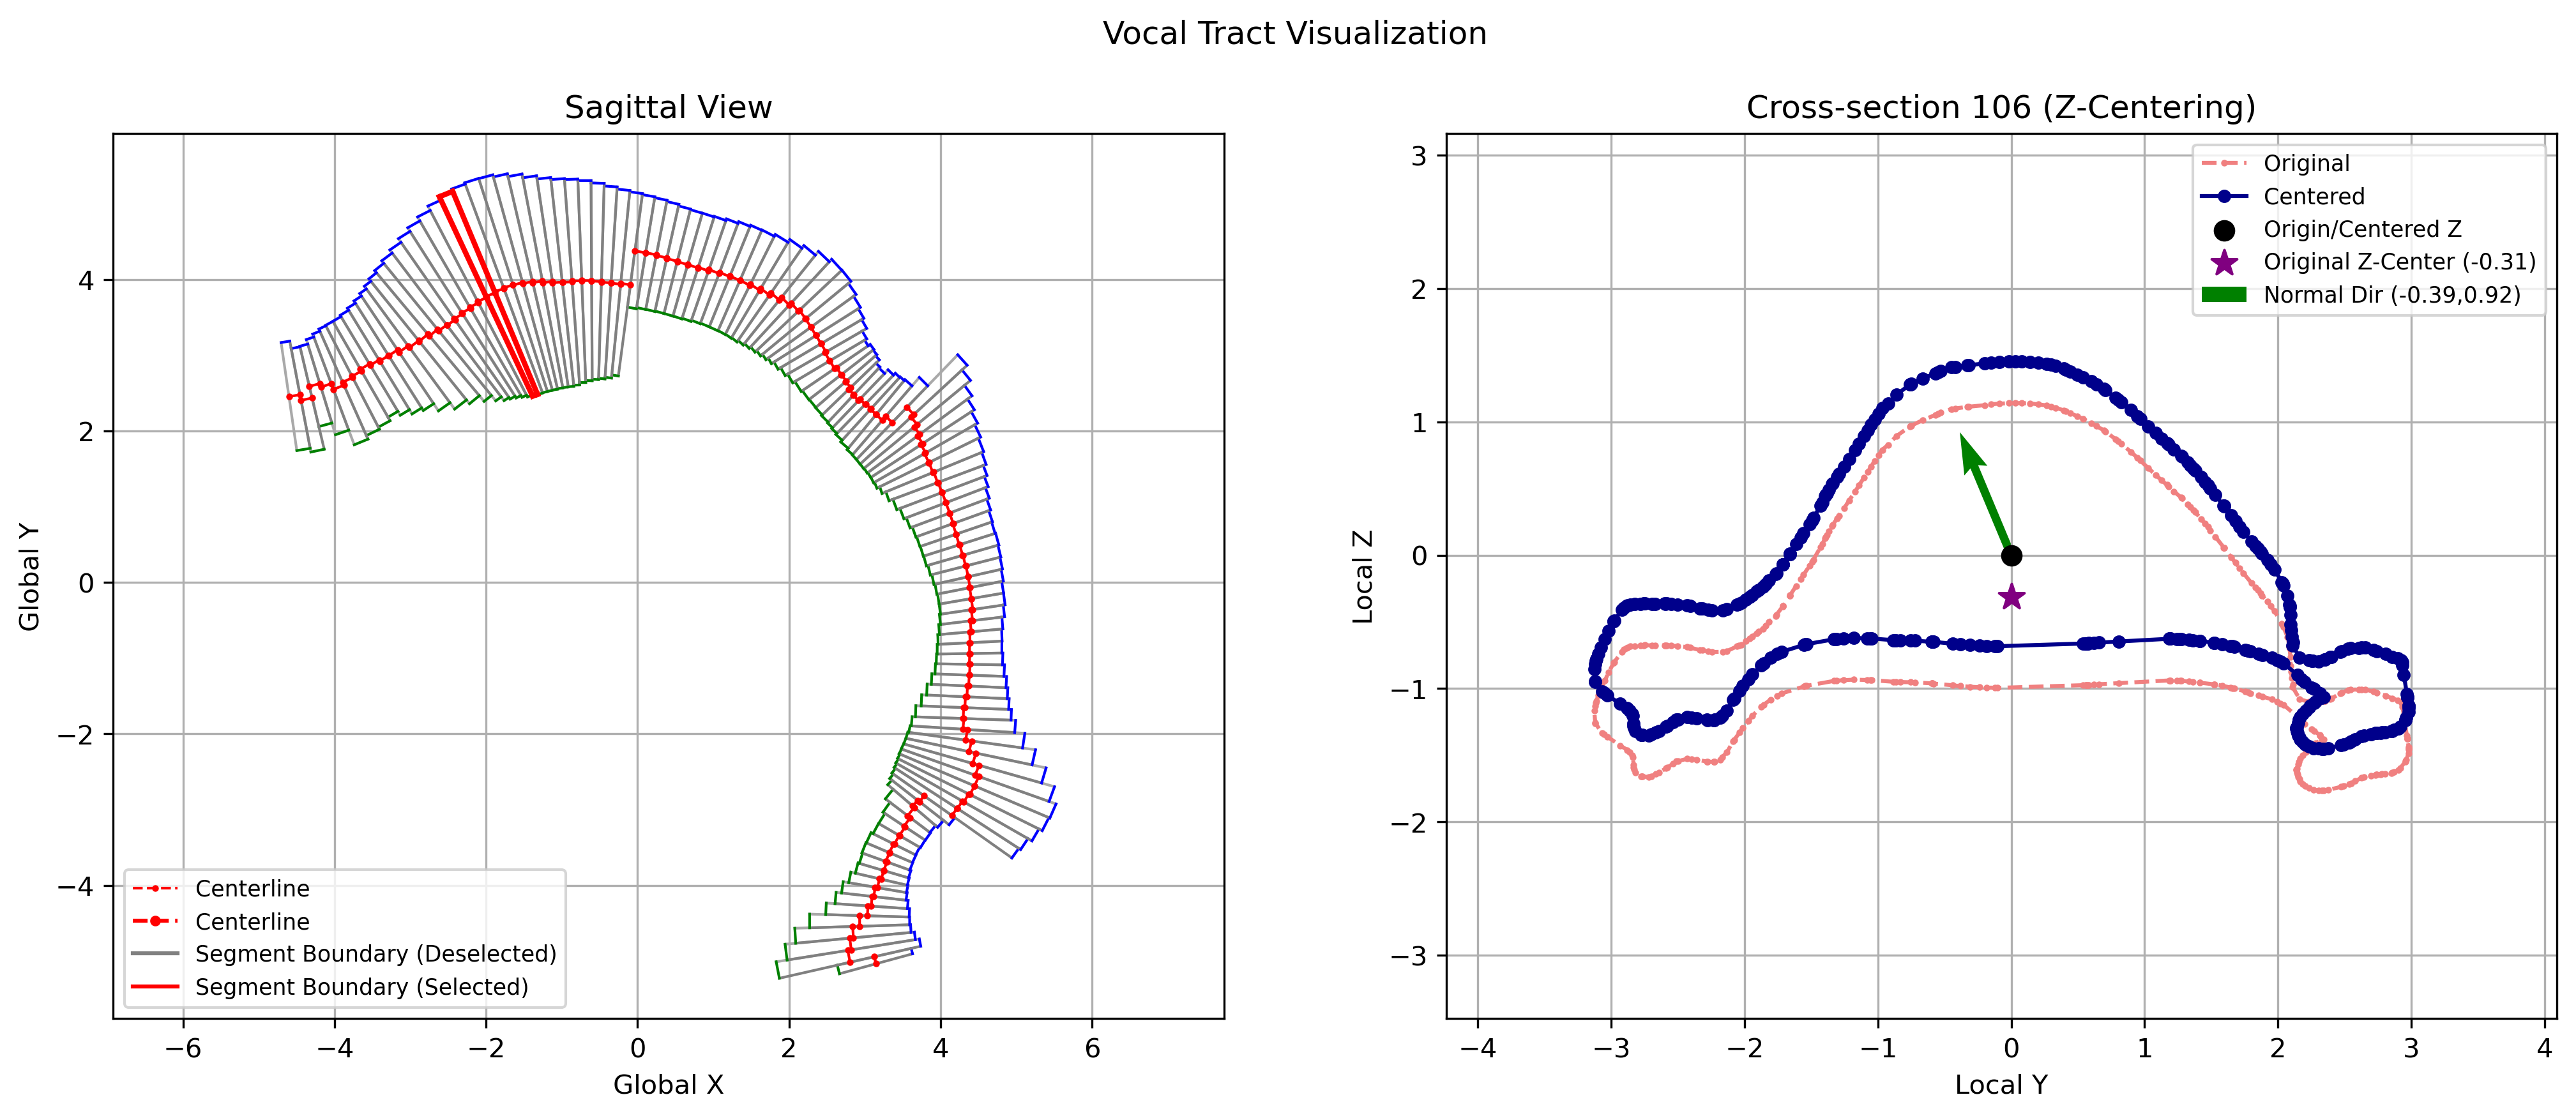
\includegraphics[width=0.6\textwidth]{contour_s1_a_plot_seg106.png}
  \caption{截面 102 的 Z 轴居中效果示意图 (由 Python 模拟脚本生成)。图中显示了原始局部轮廓(浅红色虚线)、原始 Z 轴中心(紫色星号)、居中后的局部轮廓(深蓝色实线)、局部坐标原点/居中后的 Z 轴中心(黑色点)以及该截面的入口法线方向(绿色箭头)。}
  \label{fig:cross_section_centering}
\end{figure}

\subsubsection{矢状面视图 (\texttt{SegmentsPicture})}
此视图(通常在 GUI 左上角)旨在展示整个声道的二维轮廓和中心线,由 \texttt{SegmentsPicture::draw} 方法 (位于 \texttt{SegmentsPicture.cpp:107}) 负责绘制。
\begin{itemize}
    \item 遍历所有段:通过 \texttt{for} 循环遍历 \texttt{m\_simu3d->numberOfSegments()},并在循环内调用 \texttt{sec = m\_simu3d->crossSection(i)} 从 \texttt{m\_crossSections} 获取第 \(i\) 个段对象。
    \item \textbf{中心线绘制:} 
        \begin{itemize}
            \item 获取入口点:调用 \texttt{sec->ctrLinePtIn()},这返回的是在 X.5 步骤中存储的、经过几何变换调整后的全局中心点 \({\mathbf{s}'}_i\)。
            \item 获取出口点:调用 \texttt{sec->ctrLinePtOut()}。这个点 \(\mathbf{s}_{out,i}\) \textbf{不是}直接存储的,而是由 \texttt{CrossSection2dFEM} 对象根据其内部存储的入口点 \({\mathbf{s}'}_i\)、入口法线 \(\hat{\mathbf{n}}_i\)、段长度 \(L_i\)、曲率半径 \(R_i\) 和曲率角度 \(\alpha_i\) \textbf{动态计算}出来的。计算逻辑通常委托给辅助函数 \texttt{Acoustic3dSimulation::ctrLinePtOut} (位于 \texttt{Acoustic3dSimulation.cpp} 约 4114 行)。其计算公式可以概括为:
                \begin{itemize}
                    \item 如果段是直的 (即 \(|\alpha_i| \approx 0\)):
                    \[ \mathbf{s}_{out,i} = {\mathbf{s}'}_i + L_i \cdot \mathbf{R}(-\pi/2) \hat{\mathbf{n}}_i \]
                    \paragraph{代码对应 (直线出口点):} (位于 \texttt{Acoustic3dSimulation.cpp} 约 4122-4125 行)
                    \begin{lstlisting}[language=C++]
if (abs(circleArcAngle) < MINIMAL_DISTANCE)
{
  theta = -M_PI / 2.; // 旋转角度,将法线转为切线
  Transformation rotate(CGAL::ROTATION, sin(theta), cos(theta));
  Transformation translate(CGAL::TRANSLATION, length * rotate(N)); // 沿切线平移 length
  return(translate(Pt)); // Pt 是入口点 s'_i, N 是入口法线 n_i
}
                    \end{lstlisting}
                    (其中 \(\mathbf{R}(-\pi/2)\) 代表将二维向量顺时针旋转 90 度(即旋转 \(-\pi/2\) 弧度)的旋转矩阵。此操作将入口法线向量 \(\hat{\mathbf{n}}_i\) 转换为该直线段的单位切线向量 \(\hat{\mathbf{t}}_i\),因此公式的含义为:出口点 = 入口点 + 长度 \(\times\) 单位切线方向)。
                    \item 如果段是弯曲的 (沿圆弧):
                    \[ \mathbf{s}_{out,i} = \mathbf{C} + \mathbf{R}(\alpha_i) ({\mathbf{s}'}_i - \mathbf{C}) \]
                    \paragraph{代码对应 (曲线出口点):} (位于 \texttt{Acoustic3dSimulation.cpp} 约 4132-4144 行,简化逻辑)
                    \begin{lstlisting}[language=C++]
else // Curved case
{
  theta = abs(circleArcAngle) / 2.;
  // 根据曲率半径和角度符号确定旋转方向
  if (/* condition based on signs of R and alpha */)
  {
    // 计算旋转变换 rotate1 (e.g., M_PI/2 - theta)
    // 计算平移变换 translate1 (基于 -2*R*sin(theta) 和 rotate1(-N))
    return(translate1(Pt));
  }
  else
  {
    // 计算旋转变换 rotate2 (e.g., theta - M_PI/2)
    // 计算平移变换 translate2 (基于 2*R*sin(theta) 和 rotate2(N))
    return(translate2(Pt));
  }
}
                    \end{lstlisting}
                    (其中 \(\mathbf{C}\) 是该段的曲率中心,\(\mathbf{R}(\alpha_i)\) 代表将二维向量(在此例中是从曲率中心指向入口点的向量 \({\mathbf{s}'}_i - \mathbf{C}\))逆时针旋转曲率角度 \(\alpha_i\) 的旋转矩阵)。
                    \textbf{说明:} % ... (Existing explanation text unchanged) ...
                \end{itemize}
            \item 绘制线段:在计算得到的入口点 \({\mathbf{s}'}_i\) 和出口点 \(\mathbf{s}_{out,i}\) 之间绘制线段(通常为红色)。
        \end{itemize}
    \item \textbf{段轮廓绘制 (梯形):} 这是关键步骤,用于可视化每个段在矢状面上的投影。
        \begin{enumerate}
            \item 获取轮廓边界框:调用 \texttt{bbox = sec->contour().bbox()} 获取居中轮廓 \(P'_i\) 的边界框,从中得到局部 Z 坐标范围 \(z'_{min,i} = \texttt{bbox.ymin()}\) 和 \(z'_{max,i} = \texttt{bbox.ymax()}\)。
            \item \textbf{计算梯形角点 (\texttt{getSegmentPts}):} 调用 \texttt{getSegmentPts} 函数 (位于 \texttt{SegmentsPicture.cpp:574})。此函数的核心是根据以下公式计算该段梯形轮廓的四个角点在全局坐标系 (X, Y) 中的坐标:
                \begin{itemize}
                    \item \textbf{入口下点 (\( \mathbf{B}_{in,i} \)):}
                    \[ \mathbf{B}_{in,i} = \underbrace{{\mathbf{s}'}_i}_{\texttt{ctrLinePtIn()}} + \underbrace{\hat{\mathbf{n}}_i}_{\texttt{normalIn()}} \cdot \underbrace{z'_{min,i}}_{\texttt{bbox.ymin()}} \cdot \underbrace{l_{0,i}}_{\texttt{scaleIn()}} \]
                    \paragraph{代码对应 (入口下点):} (位于 \texttt{SegmentsPicture.cpp} 约 578-580 行)
                    \begin{lstlisting}[language=C++]
Transformation translateInMin(CGAL::TRANSLATION,
  sec->scaleIn() * bbox.ymin() * sec->normalIn());
ptInMin = translateInMin(sec->ctrLinePtIn());
                    \end{lstlisting}
                    \item \textbf{入口上点 (\( \mathbf{T}_{in,i} \)):}
                    \[ \mathbf{T}_{in,i} = {\mathbf{s}'}_i + \hat{\mathbf{n}}_i \cdot z'_{max,i} \cdot l_{0,i} \]
                    \paragraph{代码对应 (入口上点):} (位于 \texttt{SegmentsPicture.cpp} 约 582-584 行)
                    \begin{lstlisting}[language=C++]
Transformation translateInMax(CGAL::TRANSLATION,
  sec->scaleIn() * bbox.ymax() * sec->normalIn());
ptInMax = translateInMax(sec->ctrLinePtIn());
                    \end{lstlisting}
                    \item \textbf{出口下点 (\( \mathbf{B}_{out,i} \)):}
                    \[ \mathbf{B}_{out,i} = \underbrace{\mathbf{s}_{out,i}}_{\texttt{ctrLinePtOut()} \text{(计算得到)}} + \underbrace{\hat{\mathbf{n}}_{out,i}}_{\texttt{normalOut()}} \cdot z'_{min,i} \cdot \underbrace{l_{1,i}}_{\texttt{scaleOut()}} \]
                    \paragraph{代码对应 (出口下点):} (位于 \texttt{SegmentsPicture.cpp} 约 586-588 行)
                    \begin{lstlisting}[language=C++]
Transformation translateOutMin(CGAL::TRANSLATION,
  sec->scaleOut() * bbox.ymin() * sec->normalOut());
ptOutMin = translateOutMin(sec->ctrLinePtOut());
                    \end{lstlisting}
                    \item \textbf{出口上点 (\( \mathbf{T}_{out,i} \)):}
                    \[ \mathbf{T}_{out,i} = \mathbf{s}_{out,i} + \hat{\mathbf{n}}_{out,i} \cdot z'_{max,i} \cdot l_{1,i} \]
                    \paragraph{代码对应 (出口上点):} (位于 \texttt{SegmentsPicture.cpp} 约 590-592 行)
                    \begin{lstlisting}[language=C++]
Transformation translateOutMax(CGAL::TRANSLATION,
  sec->scaleOut() * bbox.ymax() * sec->normalOut());
ptOutMax = translateOutMax(sec->ctrLinePtOut());
                    \end{lstlisting}
                \end{itemize}
                请注意,这些公式直接利用了先前几何变换(\eqref{eq:local_shift} 和 \eqref{eq:global_adjust})的结果:调整后的入口中心点 \({\mathbf{s}'}_i\) (通过 \texttt{ctrLinePtIn()} 获取),\textbf{动态计算出的出口中心点 \(\mathbf{s}_{out,i}\)} (通过 \texttt{ctrLinePtOut()} 获取),以及入口/出口法线 \(\hat{\mathbf{n}}_i, \hat{\mathbf{n}}_{out,i}\),居中轮廓的 Z 范围 \(z'_{min}, z'_{max}\) 和缩放因子 \(l_0, l_1\)。\texttt{getSegmentPts} 函数内部通过 CGAL 的平移变换来实现这些公式的计算。
            \item \textbf{绘制梯形:} 调用 \texttt{drawSegment} 函数 (位于 \texttt{SegmentsPicture.cpp:601}),该函数接收上一步计算出的四个角点坐标,将其转换为屏幕像素坐标,并使用 \texttt{wxDC::DrawLine} 绘制连接这些点的线段,形成梯形轮廓。
        \end{enumerate}
     \item \textbf{高亮显示:} 根据需要(例如标记活动段或噪声源段),可以用不同颜色重新调用 \texttt{drawSegment} 绘制特定段的轮廓。
\end{itemize}

\subsection{工作流程概览}

\subsubsection{流程图}
下面的流程图总结了从用户发起导入操作到系统准备好进行声学计算或更新显示的整个过程:
\begin{tikzpicture}[ % 新的 TikZ 代码,聚焦本章内容
    node distance=1cm and 0.8cm, % 调整垂直和水平间距
    scale=0.75, transform shape, % 调整整体缩放
    auto,
    block/.style={rectangle, draw, fill=blue!20, text width=9em, text centered, rounded corners, minimum height=2.5em, drop shadow, font=\footnotesize}, % 稍宽的块
    cloud/.style={ellipse, draw, fill=red!20, text centered, minimum height=2.5em, drop shadow, font=\footnotesize},
    decision/.style={diamond, draw, fill=green!20, text centered, aspect=1.5, drop shadow, font=\footnotesize},
    line/.style={draw, thick, color=black!50, -latex'},
    process/.style={rectangle, draw, fill=orange!20, text centered, minimum height=2.5em, drop shadow, font=\footnotesize, text width=10em}, % 稍宽的流程块
    io/.style={trapezium, trapezium left angle=70, trapezium right angle=110, draw, fill=cyan!20, text centered, minimum height=2.5em, drop shadow, font=\footnotesize, text width=9em},
    ready/.style={rectangle, draw, fill=green!20, text centered, rounded corners, minimum height=2.5em, drop shadow, font=\footnotesize, text width=9em}
    ]

    % Input
    \node [io] (csvFile) {CSV File Input (X.2)};

    % Backend Processing
    \node [process, below=of csvFile] (extractCSV) {\texttt{extractContoursFromCsvFile} (X.3)\\解析数据, 初步处理};
    \node [process, below=of extractCSV] (createCS) {\texttt{createCrossSections} (X.4)\\核心处理};
    \node [process, below=of createCS, text width=12em] (geoTransform) {几何变换 (X.4.1)\\局部居中 (Eq. \ref{eq:local_shift})\\全局调整 (Eq. \ref{eq:global_adjust})};
    \node [process, below=of geoTransform, text width=12em] (calcParams) {计算段参数 (X.4.2)\\长度, 曲率等};
    \node [process, below = of calcParams] (loop) {循环处理各段数据};
    \node [process, below = of loop] (addCS) {\texttt{addCrossSectionFEM} (X.5)\\实例化对象, 存储调整后数据};
    \node [process, below = of addCS] (storeCS) {对象添加到 \texttt{m\_crossSections}};
    \node [ready, below = of storeCS, fill=green!20, text width=11em] (dataReady) {几何数据处理完成\\(\texttt{m\_crossSections} 就绪)}; % Changed color and text

    % UI Update / Application Path - 移动到右侧与后端几何处理框中心对齐
    \node [cloud, right=5cm of csvFile, yshift=-1cm] (notifyUI) {通知 UI 更新 (或供计算使用)}; % 调整位置到右侧与csvFile对齐,并向下移动1cm
    \node [process, below= of notifyUI] (updateWidgets) {\texttt{UpdateWidgets} (GUI)};
    \node [io, below left=0.5cm and 0.2cm of updateWidgets] (drawSagittal) {绘制矢状面视图 (X.6.2)\\使用调整后数据计算角点};
    \node [io, below right=0.5cm and 0.2cm of updateWidgets] (drawCrossSec) {绘制横截面视图 (X.6.1)\\使用居中后轮廓};
    \node [cloud, below=5em of updateWidgets] (endDraw) {显示更新}; % 调整位置

    % Draw edges
    \path [line] (csvFile) -- (extractCSV);
    \path [line] (extractCSV) -- (createCS);
    \path [line] (createCS) -- (geoTransform);
    \path [line] (geoTransform) -- (calcParams);
    \path [line] (calcParams) -- (loop);
    \path [line] (loop) -- node [right, font=\tiny] {段数据} (addCS);
    \path [line] (addCS) -- (storeCS);
    % Loop back edge
    \path [line] (storeCS.east) .. controls +(2,0) and +(2,0) .. node [right, font=\tiny] {下一段} (loop.east);
    % Path from processing completion to UI notification/readiness
    \path [line] (storeCS) -- (dataReady); % Show data ready state
    
    % 使用多段折线连接后端处理到UI显示部分,避免干扰其他元素
    \path [line] (dataReady.east) -- ++(2.5,0) |- ++(0,17) -| node[pos=0.9, above, font=\tiny] {数据就绪} (notifyUI); % 使用多段折线连接

    % UI Update Flow
    \path [line] (notifyUI) -- (updateWidgets);
    \path [line] (updateWidgets) -- (drawSagittal);
    \path [line] (updateWidgets) -- (drawCrossSec);
    \path [line] (drawSagittal) |- (endDraw);
    \path [line] (drawCrossSec) |- (endDraw);

    % Node Grouping (Adjust fits)
    \node [draw, dashed, fit=(csvFile) (extractCSV) (createCS) (geoTransform) (calcParams) (loop) (addCS) (storeCS) (dataReady), label={[font=\footnotesize, yshift=0.2cm, xshift=-1.8cm]后端几何处理}] {};
    \node [draw, dashed, fit=(notifyUI) (updateWidgets) (drawSagittal) (drawCrossSec) (endDraw), label={[font=\footnotesize, yshift=-0.2cm, xshift=1.8cm]数据应用与显示}] {};

\end{tikzpicture}

\subsubsection{步骤总结}
以下是关键步骤的线性总结,对应于本节前面各小节的描述:
\begin{enumerate}
    \item \textbf{用户交互与文件选择:} 用户在 GUI 点击 "Import geometry",通过 \texttt{Acoustic3dPage::OnImportGeometry} (位于 \texttt{Acoustic3dPage.cpp:1094}) 选择 CSV 文件。
    \item \textbf{触发导入:} GUI 设置模拟状态并调用 \texttt{Acoustic3dSimulation::importGeometry} (位于 \texttt{Acoustic3dSimulation.cpp:5893})。
    \item \textbf{启动处理流程:} \texttt{importGeometry} 调用 \texttt{createCrossSections} (位于 \texttt{Acoustic3dSimulation.cpp:5121})。
    \item \textbf{CSV 解析 (X.3):} \texttt{createCrossSections} 调用 \texttt{extractContoursFromCsvFile} (位于 \texttt{Acoustic3dSimulation.cpp:4949}) 解析 CSV,提取原始几何数据(中心点、法线、缩放因子、局部轮廓点)到临时向量。
    \item \textbf{核心处理 (X.4):} \texttt{createCrossSections} 继续执行:
        \begin{itemize}
            \item \textbf{几何变换 (X.4.1):} 若 \texttt{m\_simuParams.curved} 为 true,执行局部轮廓 Z 轴居中 (公式 \eqref{eq:local_shift}) 和全局中心点补偿调整 (公式 \eqref{eq:global_adjust})。
            \item 计算其他参数(面积、边界框、段长度等)。
        \end{itemize}
    \item \textbf{对象实例化与存储 (X.5):} 循环处理每个段的数据:
        \begin{itemize}
            \item 调用 \texttt{addCrossSectionFEM} (位于 \texttt{Acoustic3dSimulation.cpp:531}),传递变换后的几何数据和参数,创建 \texttt{CrossSection2dFEM} 对象。
            \item 在对象内部或后续调用 \texttt{buildMesh} (位于 \texttt{CrossSection2d.cpp:321}),使用居中后的轮廓 (\(P'\)) 生成 FEM 网格。
            \item 将创建并网格化好的对象添加到 \texttt{m\_crossSections} 向量中。
        \end{itemize}
    \item \textbf{通知 UI 更新:} 后端处理完成,通知 GUI 刷新。
    \item \textbf{GUI 刷新与数据显示 (X.6):}
        \begin{itemize}
            \item \textbf{横截面视图 (X.6.1):} \texttt{PropModesPicture} (GUI 类) 获取活动段对象,绘制其居中轮廓 (\(P'\)) 或网格。
            \item \textbf{矢状面视图 (X.6.2):} \texttt{SegmentsPicture::draw} (位于 \texttt{SegmentsPicture.cpp:107}) 遍历所有段对象,绘制中心线 (基于 \({\mathbf{s}'}_i\) 和 \(\mathbf{s}_{out,i}\)),并通过 \texttt{getSegmentPts} (位于 \texttt{SegmentsPicture.cpp:574}) (使用 X.6.2 中的角点公式) 和 \texttt{drawSegment} (位于 \texttt{SegmentsPicture.cpp:601}) 绘制梯形轮廓。
        \end{itemize}
    \item \textbf{准备就绪:} 系统持有完整的、经过处理的声道几何表示(包含网格),可以响应 "Compute modes" 等后续操作。
\end{enumerate}

\begin{thebibliography}{9}
    \bibitem{Blandin2022}
    R. Blandin, M. Arnela, S. Félix, J.-B. Doc, and P. Birkholz, ``Efficient 3D Acoustic Simulation of the Vocal Tract by Combining the Multimodal Method and Finite Elements,'' \textit{IEEE Access}, vol. 10, pp. 69922--69938, 2022, doi: 10.1109/ACCESS.2022.3187424.
\end{thebibliography}

\end{document} 